\documentclass{article}
\usepackage{xeCJK}
\usepackage{amsmath,esint,amssymb,amsthm}
\usepackage{hyperref}
\usepackage{glossaries}
%\usepackage{pstricks-add}
\usepackage{tikz}
\usepackage[bottom]{footmisc}
\setCJKmainfont[AutoFakeBold]{SimSun}
\usepackage{bm}
\def\v#1{\overrightarrow{#1}}
\makeglossaries
\numberwithin{equation}{section}
\begin{document}
\title{笔记整理}
\author{赵丰}
\maketitle
\tableofcontents
\section{第二周第二次课}
\textbf{迹线}

某一流体质点的运动轨迹,其轨迹方程为常微分方程组$\frac{d \v{x}}{d t}=\v{v}$,
$\v{x}$为流体质点在$t$时刻的位置,同时也依赖于初始位置$\v{x_0}$(常微分方程组初值);$\v{v}=u\v{i}+v\v{j}+w\v{k}$为速度场,
每个分量都是空间位置和时间$t$的函数,
常微分方程组写成分量的形式为:
\begin{equation}\label{eq:22tr}
\begin{cases}
\frac{dx}{dt}=&u(x,y,z,t)\\
\frac{dy}{dt}=&v(x,y,z,t)\\
\frac{dz}{dt}=&w(x,y,z,t)
\end{cases}
\end{equation}
如对于如下的速度场
\begin{equation}\label{eq:w220}
(u,v,w)=(\frac{x}{1+t},y,z)
\end{equation}
$t=0$时初值条件为$(x,y,z)=(1,1,1)$,可直接求出上述常微分方程(ODE)有唯一解:
\begin{equation}
\begin{cases}
x=&1+t\\
y=&e^t\\
z=&1
\end{cases}
\end{equation}
这是关于$t$的参数曲线,可以通过消元得到$y=e^{x-1},z=1$,这是用空间两个曲面的交线表示曲线的方法。

\textbf{流线}

数学定义为
\begin{equation}
\frac{d \v{x}(s)}{d s}\times \v{v} =\v{0}
\end{equation}
上述定义在给定速度场后描述了空间这样一簇曲线,每条曲线每点的切线方向与该点的速度场方向一致。
使用向量外积的定义得到等价的定义形式
\begin{equation}\label{eq:2222st}
\frac{dx}{u(x,y,z,t)}=\frac{dy}{v(x,y,z,t)}=\frac{dz}{w(x,y,z,t)}
\end{equation}
这里时间$t$是常数。
上述方程如取$x$为自变量,可得到关于$(y(x),z(x))$的常微分方程组。
比如对$t=0$时刻\eqref{eq:w220}式给出的速度场为$(u,v,w)=(x,y,z)$,求过$(1,1,1)$点的流线即解ODE:
\begin{equation}
\begin{cases}
\frac{dy}{dx}=&\frac{y}{x}\\
\frac{dz}{dx}=&\frac{z}{x}
\end{cases}
\end{equation}
初值条件是$y(1)=1,z(1)=1$,从而有唯一解$y=x,z=x$。
可以看出,对同一个流场,流线和迹线是不同的。

但对于定常流,即$\bm{v}$不随时间变化,流线簇和迹线簇重合。比如考虑平面流场$(u,v)=(ax,-ay)$,
\eqref{eq:22tr}给出曲线簇$x=c_1e^{at},y=c_2e^{-at}$,\eqref{eq:2222st}给出曲线簇$xy=c$,它们表示同一曲线簇。

其他概念:

脉线、时间线、流管、流体线、流体面

\textbf{流体微团}


考虑一流体微团(系统)研究其变形规律:
\begin{figure}[!ht]
\def\svgwidth{8cm}
\centering
\input{deformation.eps_tex}
\caption{xz平面矩形的变形}\label{fig:221}
\end{figure}
由图\ref{fig:221}可以看到,$\v{OO'}+\v{O'B'}=\v{OB}+\v{BB'}$,
所以
\begin{align}\label{eq:22221}
\v{O'B'}=&\v{OB}+\v{BB'}-\v{OO'}\nonumber\\
=&\Delta x \v{i}+\v{v_B}\Delta t - \v{v_O} \Delta t
\end{align}
又
\begin{align*}
\v{v_B}=&\v{v}(x+\Delta x,y,z,t)\\
\v{v_O}=&\v{v}(x,y,z,t)
\end{align*}
所以\eqref{eq:22221}式化为:
\begin{equation}
\v{O'B'}=\Delta x \v{i} + \Delta x\Delta t \frac{\partial \v{v}}{\partial x}
\end{equation}
进一步设速度场$\v{v}=(u,v,w)$,则上式在直角坐标系下为:
\begin{equation}\label{eq:222}
\v{O'B'}=[(1+\frac{\partial u}{\partial x}\Delta t)\v{i}+\frac{\partial v}{\partial x}\Delta t\v{j}+\frac{\partial w}{\partial x}\Delta t\v{k}]\Delta x
\end{equation}
同样的方法可求出$\v{C'D'}$:
\begin{align*}
\v{C'D'}=&\v{CD}+\v{DD'}-\v{CC'}\\
=&\Delta x\v{i}+[\v{v}(x+\Delta x,y,z+\Delta z,t)-\v{v}(x,y,z+\Delta z,t)]\Delta t\\
=&\Delta x \v{i} +  \Delta x\Delta t \frac{\partial \v{v}}{\partial x}\\
\Rightarrow & \v{O'B'}=\v{C'D'}
\end{align*}
所以正六面体流体微团的微小变形后仍是平行六面体,其变形后的体积可用平行六面体体积公式求得。

设变形前正六面体由自$O'$出发的向量$\v{OA}=\Delta y\v{j},\v{OB}=\Delta x \v{i},\v{OC}=\Delta z \v{k}$张成,
变形后的六面体由自$O'$出发的向量$\v{O'A'},\v{O'B'},\v{O'C'}$张成,
对$xy,yz$两个表面类似的分析可以得到与\eqref{eq:222}类似的式子:
\begin{align*}
\v{O'C'}=&[\frac{\partial u}{\partial z}\Delta t\v{i}+\frac{\partial v}{\partial z}\Delta t\v{j}+(1+\frac{\partial w}{\partial z}\Delta t\v{k})]\Delta z\\
\v{O'A'}=&[\frac{\partial u}{\partial y}\Delta t\v{i}+(1+\frac{\partial v}{\partial y}\Delta t\v{j})+\frac{\partial w}{\partial y}\Delta t\v{k}]\Delta y
\end{align*}
变形前正六面体体积$\Delta \tau (t)=\Delta x\Delta y\Delta z$,
经过$\Delta t$时间变形后六面体体积使用混合积公式\cite{mixedProduct}并略去高阶小为:
\begin{equation}
\Delta \tau (t+\Delta t)=[1+(\frac{\partial \v{u}}{\partial x}+\frac{\partial \v{v}}{\partial y}+\frac{\partial \v{w}}{\partial z})\Delta t]\Delta x\Delta y\Delta z
\end{equation}
定义流体微团的瞬时\textbf{体膨胀率}为单位体积变化的速率,即
\begin{equation}
\Delta \tau'(t)=\lim_{\Delta t \to 0} \frac{\Delta \tau (t+\Delta t)-\Delta \tau (t)}{\Delta \tau (t)\Delta t}
\end{equation}
于是可以得到体膨胀率为$\nabla \cdot \v{v}$,为速度场的散度。当速度场的散度处处为0时,流体为不可压缩流体,变形前后体积不变。

类似的有\textbf{线变形率}的定义,对于$x$方向为:
\begin{equation}
\lim_{\Delta t \to 0} \frac{|\v{O'B'}|-|\v{OB}|}{|\v{OB}|\Delta t}
\end{equation}
其中使用Taylor 近似从\eqref{eq:222}式出发有:$|\v{O'B'}|\approx (1+\frac{\partial u}{\partial x}\Delta t)\Delta x$
于是可以求得$x$方向的线变形率为$\frac{\partial u}{\partial x}$,进而得到体膨胀率为三个方向线变形率之和的结论。


\textbf{流体的旋转角度}

对于流体绕$y$轴的旋转角度定义为$\v{O'B'}$相对于$\v{OB}$转过的角度与$\v{O'C'}$相对于$\v{OC}$转过的角度的平均值。
由于转角$\alpha$很小,有近似$\tan \alpha\approx \alpha$,所以由\eqref{eq:222}式
\begin{align*}
\measuredangle \left< \v{O'B'},\v{OB} \right>=&\frac{\frac{\partial w}{\partial x}\Delta t}{1+\frac{\partial u}{\partial x}\Delta t}\\
\approx & \frac{\partial w}{\partial x}\Delta t (1-\frac{\partial u}{\partial x}\Delta t)
\end{align*}
略去二阶小$(\Delta t)^2$即得到图中的$\alpha_1=\frac{\partial w}{\partial x}$,
因为顺时针方向为负,所以转角为$-\alpha_1$。同理求出图中的$\alpha_2=\frac{\partial u}{\partial z}$
所以流体绕$y$轴的旋转角度为
\begin{align}
\omega_y=&\frac{\alpha_2-\alpha_1}{2\Delta t}\nonumber\\
=&\frac{1}{2}(\frac{\partial u}{\partial z}-\frac{\partial w}{\partial x})
\end{align}

\textbf{流体的角变形率}

对于流体在$xz$平面的角变形率:
\begin{align}
\epsilon_{xz}=&\frac{\alpha_2+\alpha_1}{2\Delta t}\nonumber\\
=&\frac{1}{2}(\frac{\partial u}{\partial z}+\frac{\partial w}{\partial x})
\end{align}
% $S(V)$是流体微团变形后的表面,由Stokes公式:
% \[
% DV=\iiint\limits_{V}(\nabla \cdot \bm{u}Dt) dV
% \]
% 变形后的新体积
% 随时间的变化为$\frac{Dv}{Dt}$,

\section{第三周第一次课}
%\textbf{并矢与几何矢表示}
%设$\v{a},\v{b}$是三维空间向量$,则$\v{a},\v{b}$的几何矢为$\v{a}\v{b}$,$\v{a},\v{b}$的外积为$\v{a}\wedge \v{b}$
\textbf{流动运动学常用物理量的张量表示}

变形率张量
$\bm{S}=[s_{ij}]=\frac{1}{2}\left(\Delta \v{v}+(\Delta \v{v})^{\mathrm{T}}\right)$,类似弹性力学中的应变张量,为二阶对称张量。
反称张量$\bm{\Omega}=[\Omega_{ij}]=[\epsilon_{ijk}\omega_k]$,其中$\omega=\frac{1}{2}\Delta \times \bm{v}$
并且我们有:
\begin{equation}\label{eq:w31AS}
\nabla \v{v}=\bm{S}-\bm{\Omega}\cite{velocityGradient}
\end{equation}
其中速度梯度张量 $\nabla \v{v}=[v_{ij}]=[\frac{\partial v_i}{\partial x_j}]$
\footnote{$\bm{\Omega}$前是减号不是加号}

\textbf{运动分析}

\begin{figure}[!ht]%I can not compile this pstricks figure on my pC
\centering
%LaTeX with PSTricks extensions
%%Creator: inkscape 0.92.2
%%Please note this file requires PSTricks extensions
%\documentclass{article}
%\pagestyle{empty}
%\usepackage{pstricks-add}
%\usepackage{tikz}
%\begin{document}
%\begin{figure}
%\begin{pspicture}(0,0)(5,5)
%spatial axis xyz
%\psline{->}(2,2)(2,4)
%\psline{->}(2,2)(4,2)
%\psline{->}(2,2)(1,1)
%\rput(2,4){$y$}
%\rput(4,2){$x$}
%\rput(1,1){$z$}
% fluid particle pos
%\psline{->}(2,2)(3.2,2.7)
%\psline{->}(3.2,2.7)(3.8,3)
%\rput[b](3.1,2.7){$O$}
%\rput[b](3.9,3){$A$}
%\rput[b](3.5,2.85){$\delta \v{x}$}
%\rput[b](2.6,2.35){$\v{x}$}
%\end{pspicture}
%\end{figure}

%rewrite the above picture command with tikz
 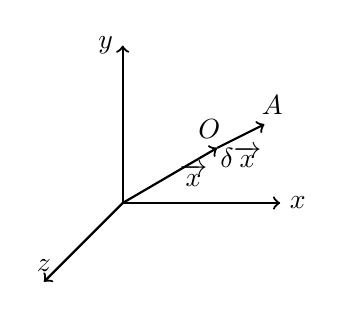
\begin{tikzpicture}
  \draw[thick,->] (2,2) -- (2,4);  
  \draw[thick,->] (2,2) -- (4,2);
  \draw[thick,->] (2,2) -- (1,1);
  \draw (2,4) node[anchor=east] {$y$};
  \draw (4,2) node[anchor=west] {$x$};
  \draw (1,1) node[anchor=south]{$z$};
  \draw (3.5,2.85) node[anchor=north] {$\delta \v{x}$};
  \draw (2.6,2.35) node[anchor=west] {$\v{x}$};
  \draw[thick,->] (2,2) -- (3.2,2.7);
  \draw[thick,->] (3.2,2.7) -- (3.8,3);
  \draw (3.1,2.7) node[anchor=south] {$O$};
  \draw (3.9,3) node[anchor=south]{$A$};
 \end{tikzpicture}
%\end{document}
\caption{流体质点从$O$点经$\Delta t$时间运动到$A$点}\label{fig:311}
\end{figure}

Helmholz 速度分解定理,参考图\ref{fig:311},有:
\begin{align}
\v{v_{A}} = & v_j(\v{x}+\delta \v{x},t)\v{e_j}\\
=& [v_j(\v{x},t)+\frac{\partial v_j}{\partial x_i}\delta x_i]\v{e_j}\\
=& [v_j(\v{x},t)+s_{ij}(\v{x},t)\delta x_i+\Omega_{ij}((\v{x},t))\delta x_i]\v{e_j}\,\footnotemark\\
=& \v{v_O} + \delta x \cdot \v{S_0} + \v{\omega_O}\times \delta \v{x}
\end{align}
\footnotetext{$\frac{\partial v_j}{\partial x_i}$是$v_{ji}$,与\eqref{eq:w31AS}不矛盾。}
其中最后一式用到了$\bm{\Omega}$和$\v{\omega}$的关系式:
\begin{equation}
\bm{\Omega} \v{x}= \v{\omega}\times \v{x} \cite{angularVelocityTensor}
\end{equation}

\newglossaryentry{vortex}
{
  name=涡量,
  description={速度场的旋量}
}
\textbf{\gls{vortex}}

定义为:$\v{\Omega}=\nabla \times \v{v}=2\v{\omega}$,其散度为零。

对于有相同流线方程的流场,其涡量场可以不同。比如流场
\begin{equation}\label{eq:31example}
\begin{cases}u=-y\\v=x\end{cases}(a) \begin{cases}u=-\frac{y}{x^2+y^2}\\v=\frac{x}{x^2+y^2}\end{cases}(b)
\end{equation}
二者的流线簇均为$x^2+y^2=c$,但$(a)$中涡量为$2\v{k}$
$(b)$中速度场在极坐标下为$\frac{\v{e_{\theta}}}{r}$,对于非原点处,
由极坐标系散度公式\cite{CylindricalCoordinates}得其散度为$\frac{\partial 1/r}{\partial \theta}=0$,
由极坐标系旋度公式\cite{CurlFormular}得涡量为$\v{0}$。
在原点处,由格林公式,速度的环量(环量积分)等于涡通量:
\begin{align}
\Gamma_l =& \oint_l \v{v}\cdot d\v{x}\\
=& \int_{0}^{2\pi} \frac{\v{e_{\theta}}}{r}\cdot  \v{e_{\theta}} rd\theta \\
=& 2\pi
\end{align}
另外不难验证$\arctan\frac{y}{x}$是后一个流场的势函数,在极坐标下其表示为$\theta$。

其他概念:

涡线、涡面、涡管

\begin{figure}[!ht]
\def\svgwidth{5cm}
\centering
\input{vortexIntensity.eps_tex}
\caption{涡通量的守恒性质}\label{fig:312}
\end{figure}



参考图\ref{fig:312},对于涡管的任一两个横截面$A_1,A_2$,有
\begin{equation}
\iint\limits_{A_1} \v{\Omega}\cdot \v{n_1} dA=\iint\limits_{A_2} \v{\Omega}\cdot \v{n_2} dA
\end{equation}
即沿涡管各截面涡通量大小相等。

\textbf{给定流场的散度与涡量求速度场}

已知区域$D$内的速度场$\v{v}$在区域内满足如下的偏微分方程(PDE):
\begin{equation}
\begin{cases}
\nabla \cdot \v{v} &=\theta (\v{x})\\
\nabla \times \v{v} &=\v{\Omega}(\v{x})\\
\end{cases}
\end{equation}
在边界上给出法向速度的大小:$\v{v}\cdot \v{n} =v_{bn}(\v{x})$
则由Poisson方程在Neumann边界条件下解的性质可以得到速度场是唯一确定的。


首先运用PDE的叠加原理将原问题分解为求如下三个PDE:
\begin{equation}\label{eq:311t3}
\begin{cases}
\nabla \cdot \v{v_E} &=\theta (\v{x})\\
\nabla \times \v{v_E} &=\v{0}\\
\end{cases}(a)
\begin{cases}
\nabla \cdot \v{v_V} &=0\\
\nabla \times \v{v_V} &=\v{\Omega}(\v{x})\\
\end{cases}(b)
\begin{cases}
\nabla \cdot \v{u} &=0\\
\nabla \times \v{u} &=\v{0}\\
\end{cases}(c)
\end{equation}
其中(\ref{eq:311t3}.c)式附加第二类边界条件$\v{u}\cdot \v{n} =v_{bn}(\v{x})-\v{v_E}\cdot \v{n}-\v{v_N}\cdot \v{n}$

对于(\ref{eq:311t3}.a),由无旋条件可知存在势场$\Phi_E$使得 $\v{v_E}=\nabla \Phi_E$,于是得到$\Phi_E$在求解区域内满足Poisson 方程:
\begin{equation}
\nabla^2 \Phi_E(\v{x})=\theta(\v{x})
\end{equation}
该方程可由三维Laplace方程的基本解$\frac{1}{|\v{x}|}$与$\theta(\v{x})$做卷积得到\cite{FundamentalSolution},写成分量的形式即为:
\begin{equation}\label{eq:31similar}
\Phi_E(x,y,z)=-\frac{1}{4\pi} \iiint\limits_D \frac{\theta(\xi,\eta,\zeta)}{R(x,y,z;\xi,\eta,\zeta)}d\xi d\eta d\zeta
\end{equation}
这里
\begin{align}
R(x,y,z;\xi,\eta,\zeta)=&|\v{R}((x,y,z;\xi,\eta,\zeta))|\\
\v{R}((x,y,z;\xi,\eta,\zeta))=&(x-\xi)\v{i}+(y-\eta)\v{j}+(z-\zeta)\v{k}
\end{align}
直接计算得到:$\nabla \frac{1}{R}=-\frac{\v{R}}{R^3}$,其中梯度算子是关于$(x,y,z)$的。
所以我们有:
\begin{equation}
\v{v_E}=\frac{1}{4\pi} \iiint\limits_D \frac{\theta(\xi,\eta,\zeta)\v{R}}{R^3}d\xi d\eta d\zeta
\end{equation}
比如散度场$\theta$为$\delta$函数,可以得到点源诱导的速度场为:
\begin{equation}
\v{v_E}=\frac{1}{4\pi} \frac{x\v{i}+y\v{j}+z\v{k}}{(x^2+y^2+z^2)^{3/2}}
\end{equation}
这与万有引力场和点电荷诱导的静电场形式相同。

对于(\ref{eq:311t3}.b),难以得到一般条件下的闭式解,因此对涡量$\Omega$在求解域的边界上附加条件
\begin{equation}\label{eq:31supp}
\v{\Omega}\cdot \v{n}=0
\end{equation}
为此,我们先用张量分析的$\epsilon-\delta$恒等式$\epsilon_{ilm}\epsilon_{ijm}=\delta_{jl}\delta_{mn}-\delta_{mj}\delta_{ln}$证明如下的等式:
\begin{equation}\label{eq:312times}
\nabla \times(\nabla \times \v{A})=\nabla(\nabla \cdot \v{A})-\nabla\cdot(\nabla \v{A})
\end{equation}
\begin{proof}
\begin{align*}
\nabla \times(\nabla \times \v{A}) =& \nabla (\epsilon_{ijk} \frac{\partial A_k}{\partial x_j} \v{e_i})\\
=&\epsilon_{nmi} \frac{\partial (\epsilon_{ijk} \frac{\partial A_k}{\partial x_j})}{\partial x_m} \v{e_n}\\
=&(\delta_{nj}\delta_{mk}-\delta{nk}\delta_{mj})\frac{\partial^2 A_k}{\partial x_j^2}\v{e_n}\footnotemark\\
=&(\frac{\partial^2 A_k}{\partial x_n^2}\v{e_n})-(\frac{\partial^2 A_n}{\partial x_j^2}\v{e_n})\\
=&(\frac{\partial}{\partial x_n}(\frac{\partial A_k}{\partial x_n})\v{e_n})-(\frac{\partial}{\partial x_k}(\frac{\partial A_n}{\partial x_j}\v{e_n}\v{e_j})\cdot \v{e_k})\\
=&(\frac{\partial}{\partial x_n}(\nabla\cdot \v{A})\v{e_n})-(\frac{\partial}{\partial x_j}(\nabla \v{A})\cdot \v{e_j})\\
=&\nabla(\nabla \cdot \v{A})-\nabla\cdot(\nabla \v{A})
\end{align*}
\footnotetext{$\frac{\partial^2 A_k}{\partial x_j^2}\v{e_n}$是对$A$的各个分量求Laplace,相当于对矢量$A$先求梯度再求散度。}
\end{proof}
运用上面的等式,我们推导 \textbf{Biot-Savart 定律}:

首先假设 (\ref{eq:311t3}.b) 中 $\v{v_V}$可以写成$\v{v_V}=\nabla \times \v{A}$,则(\ref{eq:311t3}.b)中第一式自然满足,而第二式由\eqref{eq:312times}式可化为:
\begin{equation}\label{eq:31AAA}
\nabla(\nabla \cdot \v{A})-\nabla\cdot(\nabla \v{A})=\v{\Omega}
\end{equation}
下面我们证明对于区域$D$,不考虑边界条件,\eqref{eq:31AAA}的一个解为:
\begin{equation}
\v{A}=\frac{1}{4\pi} \iiint\limits_D \frac{\v{\Omega}(\xi,\eta,\zeta)}{R(x,y,z;\xi,\eta,\zeta)} d\xi d\eta d\zeta
\end{equation}
\begin{proof}
首先证明$\nabla \cdot \v{A}=0$,记$\nabla$是关于$(x,y,z)$求梯度,而$\nabla'$是关于$\xi,\eta,\zeta$求梯度,于是有:
\begin{align*}
\nabla \cdot \v{A} =& \frac{1}{4\pi} \iiint\limits_D \v{\Omega}(\xi,\eta,\zeta)\cdot \nabla(\frac{1}{R}) d\xi d\eta d\zeta\\
=&-\frac{1}{4\pi} \iiint\limits_D \v{\Omega}(\xi,\eta,\zeta)\cdot \nabla'(\frac{1}{R}) d\xi d\eta d\zeta\\
=&-\frac{1}{4\pi} \iiint\limits_D \nabla'\cdot(\frac{\v{\Omega}}{R}) d\xi d\eta d\zeta \footnotemark\\
=&-\frac{1}{4\pi} \iint\limits_{\partial D} \frac{\v{\Omega}\cdot \v{n}}{R} dS\\
=&0\,\,(\text{由式}\eqref{eq:31supp})
\end{align*}
另一方面,与\eqref{eq:31similar}式类似,由基本解与$\Omega$做卷积得到:
\begin{equation}
-\nabla\cdot(\nabla \v{A})=\v{\Omega}
\end{equation}
从而我们得到了\eqref{eq:31AAA}式的一个特解。
\end{proof}
因此对于无散有旋的情形(\ref{eq:311t3}.b),我们得到速度场为:
\begin{align}
\v{v_V}=&\frac{1}{4\pi} \iiint\limits_D \nabla(\frac{1}{R}) \times \v{\Omega} d\xi d\eta d\zeta\\
=&\frac{1}{4\pi} \iiint\limits_D  \frac{\v{\Omega} \times \v{R}}{R^3}d\xi d\eta d\zeta \label{eq:31biotsavart}
\end{align}
以\textbf{直线涡诱导的速度场}为例,考虑一空间涡量场为:
\begin{equation}
\v{\Omega}\cdot \v{k}=\begin{cases}
\infty, & (0,0,z)\\
0, & \text{otherwise}
\end{cases}
\end{equation}
其余两个方向分量为零,并且涡通量为常数$\Gamma$,即对于区域$A_{\epsilon}(k)=\{(x,y,z)|x^2+y^2<\epsilon,z=k\}$,有
\begin{equation}
\iint\limits_{A_{\epsilon}(k)} \v{\Omega}\cdot \v{n} dS=\Gamma
\end{equation}
可以求出上述直线涡产生的速度场沿$z$轴方向不变,对于其$x,y$平面内的速度场,与式(\ref{eq:31example}.b)描述的相同。
下面用\eqref{eq:31biotsavart}式直接求该速度场,这里$D=\mathbb{R}^3$,代表全空间:
\begin{align*}
\v{v_V}=&\frac{1}{4\pi} \iiint\limits_D  \frac{\v{\Omega} \times \v{R}}{R^3}d\xi d\eta d\zeta, \,\,\text{化为累次积分,先算}\xi,\eta\\
=&\frac{1}{4\pi} \int_{\mathbb{R}}(\iint\limits_{A_{\epsilon}(\zeta)}\frac{\v{\Omega} \times \v{R}}{R^3}d\xi d\eta )d\zeta, \,\,\epsilon\text{ 可任意小}\\
=&\frac{1}{4\pi} \int_{\mathbb{R}}\left(\frac{\Gamma \v{k}\times \v{R'}}{R'^3}\right)d\zeta, R'=R(x,y,z;0,0,\zeta)\\
=&\frac{\Gamma}{4\pi} \int_{\mathbb{R}}\left(\frac{x\v{j}-y\v{i}}{(x^2+y^2+(z-\zeta)^2)^{\frac{3}{2}}}\right)d\zeta\\
=&\frac{\Gamma}{2\pi}\frac{-y\v{i}+x\v{j}}{x^2+y^2}\\
\end{align*}


\section{第四周第一次课}

针对式(\ref{eq:311t3}.c),结合附加的第二类边界条件,由无旋条件,
我们设$\v{u}=\nabla \phi$,则$\phi$满足Neumann边界条件的PDE:
\begin{equation}\label{eq:41t3}
\begin{cases}
\nabla ^2 \phi = & 0 \\
\frac{\partial \phi}{\partial \v{n}}|_{bn}= & v_{bn}(\v{x})-\v{v_E}\cdot \v{n}-\v{v_N}\cdot \v{n}\\
\end{cases}
\end{equation}
其中$\v{v_E},\v{v_N}$是(\ref{eq:311t3}.a),(\ref{eq:311t3}.b)的特解。
方程\eqref{eq:41t3}可以使用格林函数法求解\cite{GreenFunction},

\textbf{流体动力学积分型方程}

\textbf{质量体} 的边界是随时间变化的,而\textbf{控制体} 的边界是不变的。
\textbf{Reynolds 输运}定理是联系质量体和控制体的桥梁,可以把关于质量体的守恒定律轻松转化为关于控制体的守恒定律。
它的陈述为:某一质量体的某一物理量在某时刻的随体导数等于该时刻相同体积相同形状的控制体该物理量的局部导数与该物理量的通过
该控制体的表面输运量。

下面设物理量为$Q$,时刻为$t_0$, 用$D^*(t)$表示质量体,而用$D$表示$D^*(t_0)$,$\Sigma$表示$D$的边界曲面,$\v{v}$是流体速度场,$d\tau$表示体积微元。则有
\begin{equation}
\frac{D}{Dt}[\iiint\limits_{D^*(t)}Qd\tau]_{t=t_0}=\iiint\limits_{D}\frac{\partial Q}{\partial t} d\tau + \oiint\limits_{\Sigma} Q\v{v}\cdot\v{n}dA
\end{equation}

下面给出两种推导,
\begin{align*}
\frac{D}{Dt}[\iiint\limits_{D^*(t)}Q(\v{x},t)d\tau] = & \iiint\limits_{D^*(t)} \frac{D}{Dt}[Q(\v{x},t)d\tau] \\
= & \iiint\limits_{D^*(t)} [\frac{DQ}{Dt}d\tau+Q\frac{D(d\tau)}{Dt}] \\
= & \iiint\limits_{D^*(t)} [\frac{DQ}{Dt}+Q\nabla \cdot \v{v}]d\tau, \,\,\text{体膨胀率的定义}\\
= & \iiint\limits_{D^*(t)} [\frac{\partial Q}{\partial t} + \v{v} \cdot \nabla Q +Q \nabla \cdot \v{v} ] d\tau \\
= & \iiint\limits_{D} \frac{\partial Q}{\partial t}d\tau + \iiint\limits_{D^*(t)} \nabla\cdot(Q\v{v})d\tau\\
= & \iiint\limits_{D} \frac{\partial Q}{\partial t}d\tau + \oiint\limits_{\Sigma} Q\v{v}\cdot \v{n} dA, \,\,\text{Gauss 公式}
\end{align*}

另一个推导要结合图示和一些几何直观,如图\ref{fig:412}所示:

\begin{figure}[!ht]
\centering
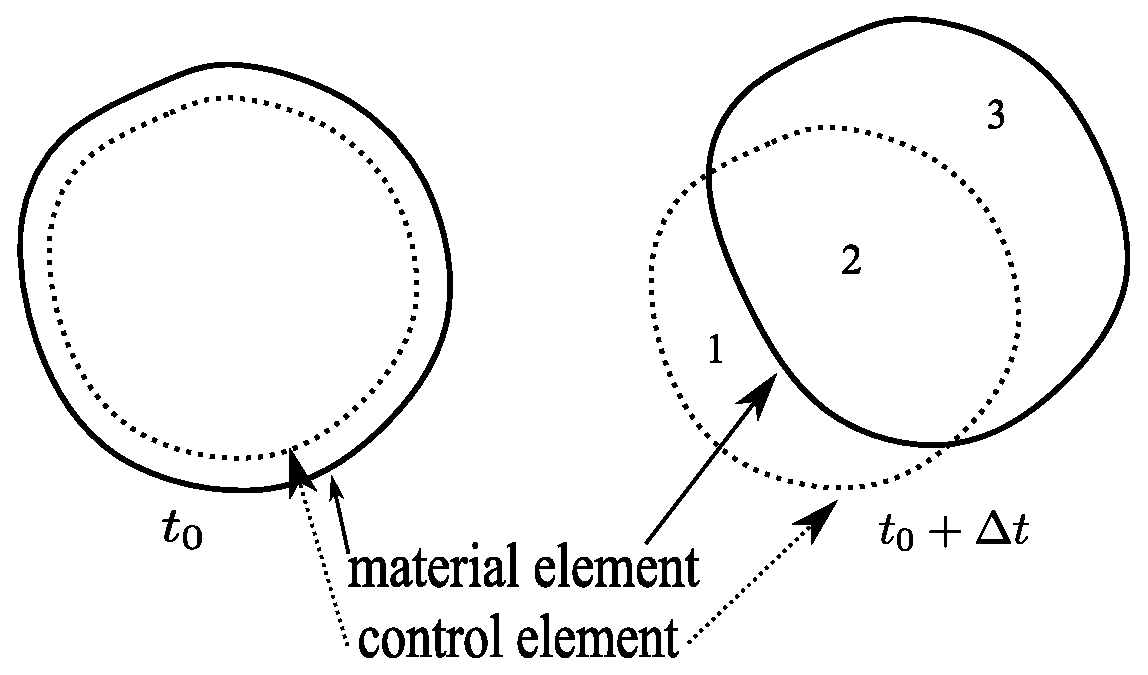
\includegraphics[width=5cm]{reynolds_derivation_illustration.eps}
\caption{雷诺输运方程推导图示}\label{fig:412}
\end{figure}
首先由随体导数的定义:
\begin{equation}
\frac{D}{Dt}[\iiint\limits_{D^*(t)}Qd\tau]_{t=t_0}=\lim_{\Delta t \to 0} \left[\frac{\iiint\limits_{D^*(t_0+\Delta t)}Q(\v{x},t_0+\Delta t) d\tau - \iiint\limits_{D^*(t_0)} Q(\v{x},t_0) d\tau  }{\Delta t}\right]
\end{equation}
积分区域$D^*(t_0+\Delta t)$可以写成$(1+2)+(3-1)$,数字所代表的区域如图\ref{fig:412}所示,注意到(1+2)仍表示控制体描述的区域,与$t_0$时刻相同,所以我们
进一步有:
\begin{align}\label{eq:41reynoldsD}
\frac{D}{Dt}[\iiint\limits_{D^*(t)}Qd\tau]_{t=t_0}=&\lim_{\Delta t \to 0} \left[
\frac{\iiint\limits_{D^*(t_0)}Q(\v{x},t_0+\Delta t) d\tau - \iiint\limits_{D^*(t_0)} Q(\v{x},t_0) d\tau  }{\Delta t}
\right]\nonumber\\
+&\lim_{\Delta t \to 0}\left[\frac{\iiint\limits_{D^*_3(t_0+\Delta t)}Q(\v{x},t_0+\Delta t) d\tau - \iiint\limits_{D^*_1(t_0+\Delta t)} Q(\v{x},t_0+\Delta t) d\tau  }{\Delta t}
\right]\nonumber\\
=& \iiint\limits_{D^*(t_0)}\frac{\partial Q}{\partial t} d\tau + \oiint\limits_{\Sigma} Q\v{v} \cdot \v{n} dA
\end{align}
式\eqref{eq:41reynoldsD}中第一项由于控制体的体积形状不变,所以对时间求导数可以挪到积分号里面;第二项根据问题的几何性质,
从1到3的体积变化由表面的流量引起,所以可以将体积的瞬时变化率转换为面积分的形式。

Reynolds 输运公式中取$Q$为不同的物理量,可以将Lagrange观点下的守恒方程(关于质量体)转化为Euler观点下的守恒方程(关于控制体)。

\textbf{质量守恒积分方程}:令$Q=$密度$\rho$,该守恒方程对任意坐标系均成立,对于质量体有:
\begin{equation}
\frac{D}{Dt} \iiint\limits_{D^*(t)}\rho d\tau =0
\end{equation}
应用Reynolds输运公式得到,对于控制体的质量守恒方程为
\begin{equation}
\iiint\limits_{D}\frac{\partial \rho}{\partial t} d\tau = - \oiint\limits_{\Sigma} \rho \v{v}\cdot \v{n} dA
\end{equation}
即控制体内质量的变化等于从控制体表面流过的质量。

我们把质量守恒定律应用于定常流,即$\frac{\partial}{\partial t}=0$,从而得到
\begin{equation}
\oiint\limits_{\Sigma} \rho \v{v}\cdot \v{n} dA
\end{equation}
对于流管,其侧面密度流量为零,如下图所示:
\begin{figure}[!ht]
\def\svgwidth{5cm}
\centering
\input{streamTube.eps_tex}
\caption{定常流流管流量守恒的性质}\label{fig:41ST}
\end{figure}

我们有
\begin{equation}
\iint\limits_{A_1} \rho\v{v}\cdot \v{n_1} dA=-\iint\limits_{A_2} \rho\v{v}\cdot \v{n_2} dA
\end{equation}

若流动是均匀的,则有$\rho_1 v_{1n} A_1 = \rho_2 v_{2n} A_2$,其中 $v_{in}$表示面$A_i$法向的速度分量。


\textbf{动量守恒积分方程}:令$Q=\rho\v{v}$(矢量),
对于质量体,我们有
\begin{equation}
\frac{D}{Dt}\iiint\limits_{D^*(t)} \rho \v{v} d\tau = \iiint\limits_{D^*(t)} \rho \v{f} d\tau + 
\oiint\limits_{\Sigma^*(t)} \rho \v{T_n} dA
\end{equation}
应用Reynolds输运公式得到,对于控制体的动量守恒方程为

\begin{equation}
\iiint\limits_{D}\frac{\partial (\rho\v{v})}{\partial t} d\tau = - \oiint\limits_{\Sigma} (\v{v}\cdot \v{n})\rho \v{v} dA +
\iiint\limits_{D^*(t)} \rho \v{f} d\tau + 
\oiint\limits_{\Sigma^*(t)} \rho \v{T_n} dA
\end{equation}

\textbf{动量矩守恒积分方程}:令$Q=\rho(\v{r} \times \v{v})$(矢量),
对于质量体,我们有
\begin{equation}
\frac{D}{Dt}\iiint\limits_{D^*(t)} \rho(\v{r} \times \v{v}) d\tau = \iiint\limits_{D^*(t)} \rho (\v{r}\times \v{f}) d\tau + 
\oiint\limits_{\Sigma^*(t)} \rho (\v{r} \times \v{T_n}) dA
\end{equation}
应用Reynolds输运公式得到,对于控制体的动量矩守恒方程为

\begin{equation}
\iiint\limits_{D}\frac{\partial}{\partial t}\rho(\v{r} \times \v{v}) d\tau = 
-\oiint\limits_{\Sigma^*(t)} \rho (\v{v} \cdot \v{n})\v{r} \times \v{v} dA+
 \iiint\limits_{D^*(t)} \rho (\v{r}\times \v{f}) d\tau + 
\oiint\limits_{\Sigma^*(t)} \rho (\v{r} \times \v{T_n}) dA
\end{equation}


\textbf{能量守恒积分方程}:令$Q=\rho(e+\frac{1}{2}|\v{v}|^2)$,$e$是单位质量流体的内能
\begin{equation}
\frac{D}{Dt}\iiint\limits_{D^*(t)} \rho(e+\frac{1}{2}|\v{v}|^2) d\tau = \iiint\limits_{D^*(t)} \rho \v{f}\cdot\v{v} d\tau + 
\oiint\limits_{\Sigma^*(t)} \rho \v{T_n}\cdot\v{v} dA + \iiint\limits_{D^*(t)}\rho (\dot{q}+q_R)d\tau +
\oiint\limits_{\Sigma^*(t)} \lambda \v{n}\cdot \nabla T dA
\end{equation}
应用Reynolds输运公式即可将上述方程改写为控制体的形式,这里略去。

\section{第四周第二次课}

下面我们针对两组假设条件下的能量守恒积分方程进行化简:
第一组假设
\begin{itemize}
\item 理想流体,即表面力为 $T_n=-p \v{n}$
\item 有势场,即存在标量函数$\Pi$, 使得$\v{f}=-\nabla \Pi$
\item 绝热
\item 定常流,即流体任意物理量$Q$只与空间坐标有关,与时间无关,
满足$\frac{\partial Q}{\partial t}=0$
\end{itemize}

在第一组假设下,能量守恒积分方程可化为
\begin{equation}\label{eq:42energy}
\oiint\limits_{\Sigma} \rho (e+\frac{1}{2}|\v{v}|^2)\v{v}\cdot\v{n} dA +
\iiint\limits_{D} \rho (\nabla \Pi)\cdot \v{v} d\tau 
+ \oiint\limits_{\Sigma} p \v{n}\cdot\v{v}dA=0
\end{equation}
我们尝试把上式第二项的体积分化为面积分,为此用到:
\begin{align*}
\rho (\nabla \Pi)\cdot \v{v} = & \nabla \cdot (\Pi \rho \v{v}) - \Pi \nabla \cdot(\rho \v{v})\\
= & \nabla \cdot (\Pi \rho \v{v}) \quad \text{定常流的连续性方程}
\end{align*}
因此我们得到
\begin{equation}
\oiint\limits_{\Sigma} \rho[\Pi + \frac{p}{\rho} + e + \frac{1}{2} |\v{v}|^2](\v{v}\cdot \v{n})dA=0
\end{equation}
上式中第一项$\Pi$表示体积势的贡献,第二项和第三项之和表示焓(内能与压力势之和),最后一项表示动能。

如果我们取$D$是一个流管,如图\ref{fig:412}所示,侧面积分为零,因此我们有
\begin{equation}
\oiint\limits_{A_1} \rho[\Pi + \frac{p}{\rho} + e + \frac{1}{2} |\v{v}|^2](\v{v}\cdot \v{n})dA=
-\oiint\limits_{A_2} \rho[\Pi + \frac{p}{\rho} + e + \frac{1}{2} |\v{v}|^2](\v{v}\cdot \v{n})dA
\end{equation}
假设面积$A_1,A_2$很小流动可以看作均匀的,从而
\begin{equation}
\rho[\Pi_1 + \frac{p_1}{\rho_1} + e_1 + \frac{1}{2} |\v{v_1}|^2](\v{v_1}\cdot \v{n_1})A_1=
-\rho[\Pi_2 + \frac{p_2}{\rho_2} + e_2 + \frac{1}{2} |\v{v_2}|^2](\v{v_2}\cdot \v{n_2})A_2
\end{equation}
代入微元流管的连续性方程
$\rho(\v{v}\cdot \v{n})A_1=-\rho(\v{v}\cdot \v{n})A_2$,我们得到
\begin{equation}
\Pi_1 + \frac{p_1}{\rho_1} + e_1 + \frac{1}{2} |\v{v_1}|^2 = \Pi_2 + \frac{p_2}{\rho_2} + e_2 + \frac{1}{2} |\v{v_2}|^2
\end{equation}
因此沿流线,我们得到第一组假设下的Bernoulli方程
\begin{equation}
\Pi + \frac{p}{\rho} + e + \frac{1}{2} |\v{v}|^2=c
\end{equation}
第二组假设
\begin{itemize}
\item 理想流体,即表面力为 $T_n=-p \v{n}$
\item 有势场,即存在标量函数$\Pi$, 使得$\v{f}=-\nabla \Pi$
\item 不可压缩条件,即流体微团体积不随时间变化 $\frac{D \rho}{D t}=0$
\item 定常流,即流体任意物理量$Q$只与空间坐标有关,与时间无关,满足$\frac{\partial Q}{\partial t}=0$
\end{itemize}
在第二组假设下,由于体膨胀作功的部分为零,由热力学第一定律,内能的变化只与热交换有关,
因此在能量守恒方程中我们可以将内能与热交换项分离出来,从而得到\eqref{eq:42energy}式,但此时$e=0$,
类似的化简得到在第二组假设下的Bernoulli方程
\begin{equation}
\Pi + \frac{p}{\rho} + \frac{1}{2} |\v{v}|^2 = c
\end{equation}
进一步假设有势场是重力场,即$\Pi=gz$,$z$代表高度方向坐标,则得到Bernoulli方程的常用形式:
\begin{equation}
gz + \frac{p}{\rho} + \frac{1}{2} |\v{v}|^2 = c
\end{equation}

\begin{equation}
\end{equation}

\section{第五周第一次课}

积分型守恒方程应用的两个例子

1.流体对水平弯管的作用力
\begin{figure}[!ht]
\centering
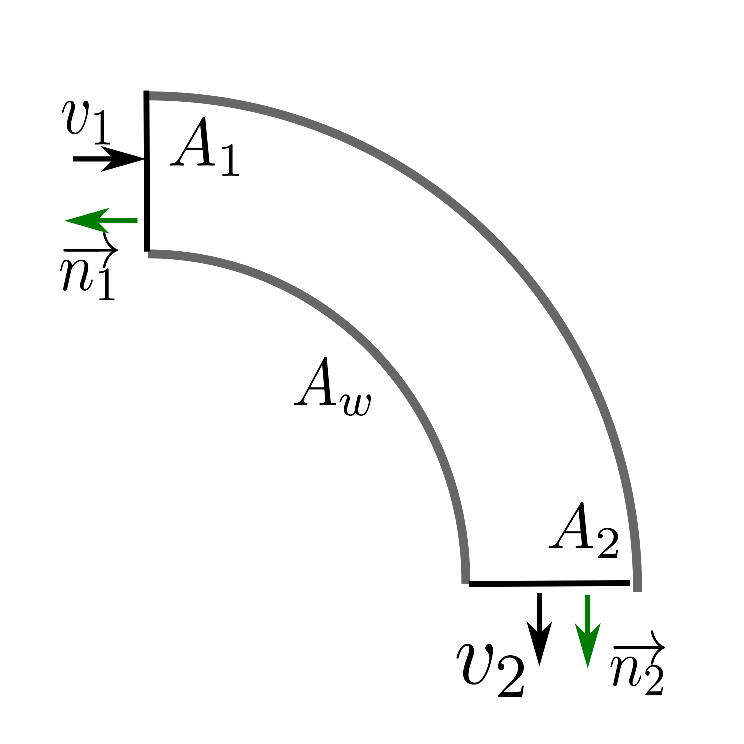
\includegraphics[width=5cm]{horizontal_tube.eps}
\caption{水平弯管}\label{fig:511}
\end{figure}

如上图所示,已知管的入口横截面和出口横截面面积分别为$A_1$,$A_2$。
进水口速度为$v_1$,压强为$p_1$,流体假设为理想不可压定常流,密度为$\rho$,求流体对水平弯管的作用力。

解:坐标系选为地面系,控制体选为水平弯管,由连续性方程有:
\begin{equation}\label{eq:51H1}
v_1A_1=v_2A_2
\end{equation}
由Bernoulli方程有:
\begin{equation}\label{eq:51H2}
\frac{1}{2}v_1^2+\frac{p_1}{\rho}=\frac{1}{2}v_2^2+\frac{p_2}{\rho}
\end{equation}
由动量守恒积分方程
\begin{equation*}
\oiint\limits_{\Sigma} \v{T_n} dA+\iiint\limits_{\tau}\rho\v{f}\d\tau
-\oiint\limits_{\Sigma}\rho\v{v}(\v{v}\cdot\v{n})dA=0
\end{equation*}
上式中$T_n$是表面力,在$A_i$面上($i=1,2$),由于$T_n=-p_i\v{n_i}$,而在$A_w$面上,设所求的作用力为$\v{F}$则弯管对流体的
作用力为$-\v{F}$,因此第一项化简为$-\v{F}-p_1A_1\v{n_1}-p_2A_2\v{n_2}$。
上式第二项为体积力的贡献,即为重力势$\rho \v{g} \tau$,其中$\tau$为管内流体体积。
上式第三项为动量的输运项,考虑到$\v{v_1}=-v_1\v{n_1},\v{v_2}=v_2\v{n_2}$,可得到第三项(不带前面负号)为
$\rho v_1^2 A_1\v{n_1}+\rho v_2^2 A_2\v{n_2}$,因此动量守恒方程最终化为
\begin{equation}\label{eq:51H3}
\v{F}=\rho g \tau -p_1A_1\v{n_1}-p_2A_2\v{n_2} - \rho v_1^2 A_1\v{n_1} - \rho v_2^2 A_2\v{n_2}
\end{equation}
从式\eqref{eq:51H1}和式\eqref{eq:51H2}中解出$v_2,p_2$代入式\eqref{eq:51H3}中得到流体对水平弯管的作用力为:
\begin{equation}
\v{F}=\rho \v{g} \tau -p_1A_1\v{n_1}-(\frac{\rho v_1^2}{2}-\frac{\rho v_1^2A_1^2}{2A_2^2}+p_1)A_2\v{n_2} - \rho v_1^2 A_1\v{n_1} - \rho \frac{v_1^2A_1^2}{A_2^2} A_2\v{n_2}
\end{equation}
若$A_1=A_2$,则可推出$v_1=v_2,p_1=p_2$,作用力化简为:
\begin{equation}
\v{F}=\rho \v{g} \tau -(p_1+\rho v_1^2)(\v{n_1}+\v{n_2})
\end{equation}
由于$\v{g}$与水平弯管平面垂直,当$\v{n_1}=-\v{n_2}$,即管是直的,作用力达到最小,这对消防员灭火时使用喷水管的方法具有一定指导意义。

2.叶轮机械的功率
\begin{figure}[!ht]
\centering
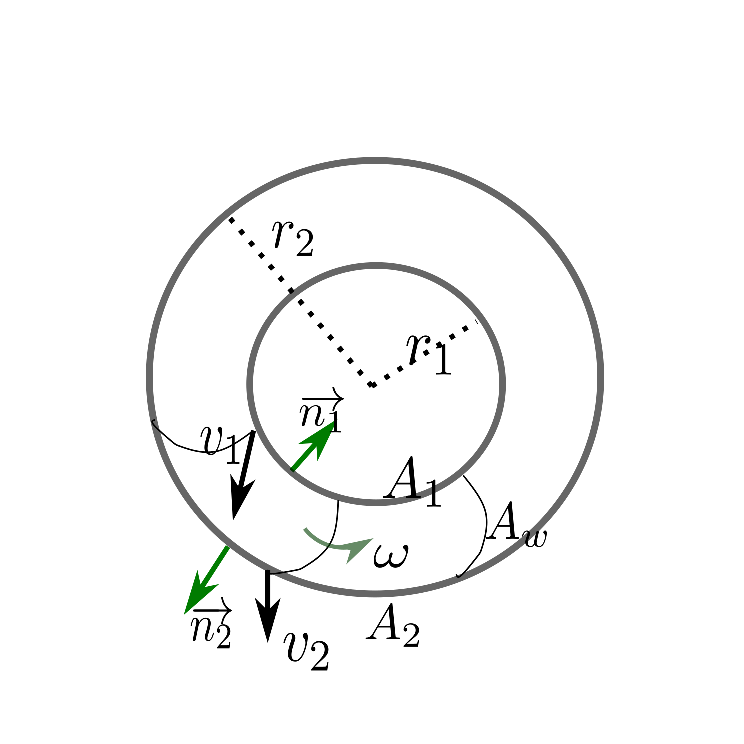
\includegraphics[width=5cm]{turbine_power.eps}
\caption{叶轮机械示意图}\label{fig:512}
\end{figure}

叶轮机械的简化模型如上图所示,转动角速度为常数$\v{\omega}$,纵向$\v{e_z}$设为单位长度,
流体假设为理想不可压定常流,且速度分布均匀,我们取旋转中的叶轮机为参考系,
以叶轮机为控制体。由于我们选的参考系是非惯性系,需要考虑惯性力项,为此首选考虑速度的分解,设$\v{u}$是叶轮机上某位置对地速度,
$\v{w}$是该位置流体微团相对叶轮机的速度,$\v{v}$是该位置流体微团对地速度,速度分解关系如下图所示:
\begin{figure}[!ht]
\centering
%LaTeX with PSTricks extensions
%%Creator: inkscape 0.92.2
%%Please note this file requires PSTricks extensions
%\documentclass{article}
%\pagestyle{empty}
%\usepackage{tikz}
%\begin{document}
 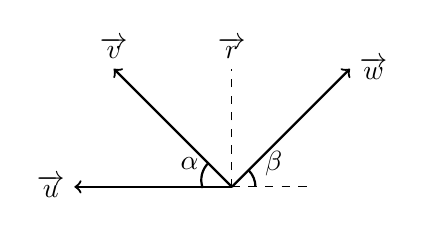
\begin{tikzpicture}
  \draw[thick,->] (2,0) -- (0,0);
  \draw[thick,->] (2,0) -- (3.5,1.5);
  \draw[thick,->] (2,0) -- (0.5,1.5);
  \draw[thick] (23mm,0mm) arc [start angle=0, end angle=45, radius=3mm]; %beta
  \draw[thick] (17mm,3mm) arc [start angle=135, end angle=200, radius=3mm]; %alpha
  \draw (0,0) node[anchor=east] {$\overrightarrow{u}$};
  \draw (3.5,1.5) node[anchor=west] {$\overrightarrow{w}$};
  \draw (0.5,1.5) node[anchor=south] {$\overrightarrow{v}$};
  \draw (1.7,0.3) node[anchor=east] {$\alpha$};
  \draw (2.3,0.3) node[anchor=west] {$\beta$};
  \draw[dashed] (2,0) -- (3,0);
  \draw[dashed] (2,0) -- (2,1.5);
  \draw (2,1.5) node[anchor=south] {$\overrightarrow{r}$};  
  \end{tikzpicture}
%\end{document}
\caption{速度分解关系示意图}\label{fig:513}
\end{figure}
且满足$\v{v}=\v{w}+\v{u}$,其中$\beta$被称为安装角,$\alpha$为进气(出气)角。该位置流体微团对地的加速度
\begin{equation}
\v{a}=\v{\omega}\times(\v{\omega}\times \v{r})+2\v{\omega}\times \v{w}
\end{equation}
化简可得:
\begin{equation}\label{eq:51acc}
-\v{a}=\omega^2 \v{r} +2\v{w}\times \v{\omega}
\end{equation}
由动量矩守恒积分方程有:

\begin{equation}\label{eq:momentumConservation}
\underbrace{\iiint\limits_D \rho(\v{r}\times (\v{f}-\v{a}))d\tau}_{I_1}+
\underbrace{\oiint\limits_{\Sigma} (\v{r}\times\v{T_n})dA}_{I_2}-
\underbrace{\oiint\limits_{\Sigma} (\v{r}\times \rho\v{w})(\v{w}\cdot\v{n})dA}_{I_3}=0
\end{equation}

\begin{align}
I_1= & \iiint\limits_D \rho(\v{r}\times (-\v{a}))d\tau, \v{f}=\v{g}\text{与叶轮机平面垂直} \nonumber\\
= & \iiint\limits_D \rho(\v{r}\times (\omega^2 \v{r} +2\v{w}\times \v{\omega}))d\tau,\text{代入}\eqref{eq:51acc}\nonumber\\
= & 2\iiint\limits_D \rho((\v{r}\cdot\v{\omega})\v{w}-(\v{r}\cdot\v{w})\v{\omega})d\tau, A\times (B\times C)=(A\cdot C)B-(A\cdot B)C\nonumber\\
= & -2\iiint\limits_D \rho (\v{r}\cdot\v{w})\v{\omega}d\tau\nonumber\\
= & -2\left(\int_{r_1}^{r_2} rdr\right)\left(\int_0^{2\pi}\rho(\v{r}\cdot\v{w})d\theta\right)\v{\omega}, \text{按柱坐标积分}\nonumber\\
= & -Q_m(\omega r_2^2-\omega r_1^2)\v{e_z}, \text{质量流量的定义}Q_m=\int_0^{2\pi}\rho(\v{r}\cdot\v{w})d\theta\nonumber\\
= & -Q_m(u_2r_2-u_1r_1)\v{e_z},\text{入口和出口处牵连速度为圆周运动线速度} \label{eq:51I1}\\
\end{align}

由于相对速度$\v{u}$沿侧面切线方向,与$\v{n}$点积为零,侧面积分为零,$I_3$中面积分只需考虑$A_1\cup A_2$,
由连续性方程:$Q_m=-\rho_1 \v{w_1}\cdot \v{n_1} A_1=\rho_2 \v{w_2}\cdot \v{n_2} A_2$。
同样由图\ref{fig:513}的几何关系,在$A_1$面上有
$\v{r}\times \v{w}=-r_1 w_1 \cos\beta_1 \v{e_z}$,
因此对$A_1$上的面积分我们有
\begin{equation}
\oiint\limits_{A_1} (\v{r}\times \rho\v{w})(\v{w}\cdot\v{n})dA=Q_m r_1 w_1 \cos\beta_1 \v{e_z}
\end{equation}
同理可求出$A_2$上的面积分为$-Q_m r_2 w_2 \cos\beta_2 \v{e_z}$,进而得到
\begin{equation}\label{eq:51I3}
I_3=Q_m (r_1 w_1 \cos\beta_1 - r_2 w_2 \cos\beta_2) \v{e_z}
\end{equation}

$I_2$包含叶片侧面对流体的力矩,通过式\eqref{eq:momentumConservation}可以求出该力矩。
由于是理想流体,$\v{T_n}=-p\v{n}$与$\v{r}$平行,因此进出口面$A_1,A_2$无力矩,于是我们得到:
\begin{align*}
\v{M}=& I_2 \\
=& -I_1+ I_3 \\
=& Q_m (u_2r_2-u_1r_1)\v{e_z} + Q_m (r_1 w_1 \cos\beta_1 - r_2 w_2 \cos\beta_2) \v{e_z}, \text{式\eqref{eq:51I1}和\eqref{eq:51I3}} \\
=& Q_m[r_2(u_2-w_2\cos\beta_2)-r_1(u_1-w_1\cos\beta_1)]\v{e_z}\\
=& Q_m(r_2v_2\cos\alpha_2 - r_1 v_1\cos\alpha_1)\v{e_z},\text{图\ref{fig:513}中几何关系} \\
\end{align*}
进一步我们可求出叶轮机的功率$N=\v{M}\cdot\v{\omega}$。

\section{第五周第二次课}

流体动力学微分型方程的建立

微分型方程在流场内部是逐点满足的,附加上流场的边界条件和初始条件,即可通过求解PDE的方法得到流场的各个参量。

微分型方程可以通过积分型方程中将面积分通过Gauss公式化为体积分,利用积分区域的任意性得到被积函数逐点成立。

1.连续方程,由\eqref{eq:41Conti}式可得到
\begin{equation}
\iiint\limits_D \left(\frac{\partial \rho}{\partial t}+\nabla\cdot(\rho \v{v})\right)d\tau=0
\end{equation}
从而得到
\begin{equation}\label{eq:52Conti}
 \frac{\partial \rho}{\partial t}+\nabla\cdot(\rho \v{v})=0
\end{equation}
或者写成
\begin{equation}\label{eq:52ContiMaterial}
 \frac{1}{\rho}\frac{D \rho}{D t}+\nabla\cdot\v{v}=0
\end{equation}
即密度增长率与体膨胀率之和为零。

1.动量方程,由\eqref{eq:41Momen}式可得到

\begin{equation}
\iiint\limits_{D}\frac{\partial (\rho\v{v})}{\partial t} d\tau =- \oiint\limits_{\Sigma} (\rho\v{v}\v{v})\cdot \v{n} dA +
\iiint\limits_{D} \rho \v{f} d\tau + 
\oiint\limits_{\Sigma} \rho \bm{T}\cdot\v{n} dA
\end{equation}
上式中$\v{v}\v{v}$是并矢的写法,$\bm{T}$是应力张量,因此我们有
\begin{equation}
\iiint\limits_{D} \frac{\partial (\rho\v{v})}{\partial t}d\tau=
\iiint\limits_{D} \left(\rho\v{f}+\nabla\cdot\bm{T}-\nabla\cdot(\rho\v{v}\v{v})\right)d\tau
\end{equation}
从而得到
\begin{equation}
 \frac{\partial (\rho\v{v})}{\partial t}=\rho\v{f}+\nabla\cdot\bm{T}-\nabla\cdot(\rho\v{v}\v{v})
 \end{equation}
利用$\nabla\cdot(\rho\v{v}\v{v})=\v{v}\nabla\cdot(\rho\v{v})+\rho\v{v}\cdot\nabla\v{v}$
\footnote{
LHS=$(\frac{\partial}{\partial x_i})\v{e_i}\cdot[\rho v_jv_k\v{e_j}\v{e_k}]
=\frac{\partial}{\partial x_i}(\rho v_iv_k)\v{e_k}
=\frac{\partial \rho v_i}{\partial x_i}v_k\v{e_k}+(\rho v_i)\frac{\partial \rho v_k}{\partial x_i}\v{e_k}
=$RHS
},
可以进一步将上式化简为
\begin{align}\notag
 \rho\frac{\partial \v{v}}{\partial t}+\underbrace{\frac{\partial \rho}{\partial t}\v{v}+\v{v}\nabla\cdot(\rho\v{v})}_{\text{by eqn }\eqref{eq:52Conti}}+\rho\v{v}\cdot\nabla\v{v}=&\rho\v{f}+\nabla\cdot\bm{T}\\
 \rho\frac{\partial \v{v}}{\partial t}+\rho\v{v}\cdot\nabla\v{v}=&\rho\v{f}+\nabla\cdot\bm{T}\label{eq:52Momen}
 \end{align}
或写成
\begin{equation}
\rho\frac{D \v{v}}{D t}=\rho \v{f} + \nabla \cdot \bm{T}
\end{equation}
由式\eqref{eq:41Energy}得到关于控制体的能量方程为:
\begin{align}\notag
\frac{\partial}{\partial t}\iiint\limits_{D} \rho(e+\frac{1}{2}|\v{v}|^2) d\tau =& \iiint\limits_{D} \rho \v{f}\cdot\v{v} d\tau + 
\oiint\limits_{\Sigma}  \v{T_n}\cdot\v{v} dA + \iiint\limits_{D}\rho (\dot{q}+q_R)d\tau \\
+&\oiint\limits_{\Sigma} \lambda \v{n}\cdot \nabla T dA-\oiint\limits_{\Sigma}\rho(e+\frac{1}{2}|\v{v}|^2)(\v{v}\cdot\v{n})dA
\end{align}
面积分化为体积分得:
\begin{align}\notag
\frac{\partial}{\partial t}\iiint\limits_{D} \rho(e+\frac{1}{2}|\v{v}|^2) d\tau =& 
\iiint\limits_{D} \rho \v{f}\cdot\v{v} d\tau + 
\iiint\limits_{D}  \nabla\cdot(\v{T_n}\cdot\v{v}) d\tau + 
\iiint\limits_{D}\rho (\dot{q}+q_R)d\tau \\
+&\iiint\limits_{D} \nabla\cdot(\lambda \v{n}\cdot \nabla T) d\tau-
\iiint\limits_{D}\nabla\cdot(\rho(e+\frac{1}{2}|\v{v}|^2)\v{v})d\tau
\end{align}
因此有
\begin{equation}
\frac{\partial}{\partial t} \rho(e+\frac{1}{2}|\v{v}|^2)  =
 \rho \v{f}\cdot\v{v}  + 
\nabla\cdot(\v{T_n}\cdot\v{v})  + 
\rho (\dot{q}+q_R) 
+\nabla\cdot(\lambda \v{n}\cdot \nabla T) -
\nabla\cdot(\rho(e+\frac{1}{2}|\v{v}|^2)\v{v})
\end{equation}
利用连续性方程\eqref{eq:52Conti}进一步化简为:
\begin{equation}\label{eq:52Energy}
\rho \frac{D(e+\frac{1}{2}|\v{v}|^2)}{Dt}=\rho \v{f}\cdot\v{v}+\nabla\cdot(\bm{T}\cdot\v{v})+\rho(\dot{q}+q_R) +\nabla\cdot(\lambda \v{n}\cdot \nabla T)
\end{equation}
角动量守恒方程可以推出应力张量$\bm{T}$是对称张量,因此对于$\bm{T}$,未知量只有6个。

上面方程(\ref{eq:52Conti},\ref{eq:52Momen},\ref{eq:52Energy})只有5个方程,但未知量有应力张量$\bm{T}$,速度场$\v{v}$,温度场$\theta$,内能$e$,密度$\rho$共12个未知量,
因此需要补充物理方程才能达到定解条件。对于牛顿流体,物理方程指出应力张量与应变张量之间是线性关系:
满足如下方程:
\begin{equation}\label{eq:52TSG}
T_{ij}=(-p+(\mu'-\frac{2}{3}\mu)\nabla\cdot \v{v})\delta_{ij}+2\mu S_{ij}
 \end{equation}
其中 $\bm{S}$是应变率张量,$S_{ij}=\frac{1}{2}(\frac{\partial v_i}{\partial x_j}+\frac{\partial v_j}{\partial x_i})$,
$\mu$是流体的动力黏性系数(viscosity),而$\mu'$是第二黏性系数。

上面补充了6个方程,但引入了一个新的变量,压强$p$,为此再补充两个热力学方程:
\begin{align}
e=&C_v\theta\\
p=&\rho R\theta,\text{对液体通常满足不可压条件,即$\rho=$Const}
 \end{align}
 这样方程与未知数的个数相等,在适当的边界条件下可以求解PDE。
 实际上对于一些特定的假设,可以适当减少方程和未知量的个数,下面针对均质不可压流做进一步化简。

 由于流体不可压,$\nabla\cdot\v{v}=0$,所以\eqref{eq:52TSG}式化简为$T_{ij}=-p\delta_{ij}+2\mu S_{ij}$,
 下面化简$\nabla\cdot \bm{T}$
\begin{align}
\nabla\cdot \bm{T} = & (\frac{\partial}{\partial x_k}\v{e_k})\cdot(T_{ij}\v{e_i}\v{e_j})\nonumber\\
= & \frac{\partial T_{ij}}{\partial x_i}\v{e_j} \label{eq:52TijUn}\\
= & \frac{\partial}{\partial x_i}(-p\delta_{ij}+2\mu S_{ij})\v{e_j}\nonumber\\
= & -\frac{\partial p}{\partial x_i}\v{e_i}+\mu \frac{\partial}{\partial x_i}(\frac{\partial v_i}{\partial x_j}+\frac{\partial v_j}{\partial x_i})\v{e_j}\nonumber\\
= & -\nabla p+\mu \frac{\partial^2 v_j}{\partial x_i^2}\v{e_j},\text{利用 }\nabla\cdot\v{v}=0\nonumber\label{eq:52nablav0C}\\
= & -\nabla p+\mu \nabla^2 \v{v}
\end{align}
 将其代入动量方程 \eqref{eq:52Momen}式,并设外力场为重力场,得到均质不可压流的N-S方程:
\begin{equation}\label{eq:52NSEqUnCompress}
\rho\frac{\partial \v{v}}{\partial t}+\rho\v{v}\cdot\nabla\v{v}=\rho\v{g}-\nabla p+\mu \nabla^2 \v{v}
 \end{equation}
 下面推导其在柱坐标系下的表达式,此时
 \begin{align}
 \nabla^2=&\frac{\partial^2 }{\partial r^2}+\frac{1}{r}\frac{\partial}{\partial r}+
 \frac{1}{r^2}\frac{\partial^2 }{\partial \theta^2}+\frac{\partial^2 }{\partial z^2}\\
 \nabla=&\v{e_r}\frac{\partial}{\partial r}+\frac{\v{e_{\theta}}}{r}\frac{\partial}{\partial \theta }+\v{e_z}\frac{\partial}{\partial z}\label{eq:52nablacy}
 \end{align}
 并利用$\frac{\partial \v{e_r}}{\partial \theta}=\v{e_{\theta}}$和$\frac{\partial \v{e_{\theta}}}{\partial \theta}=-\v{e_r}$
于是可得
 \begin{align*}
 \nabla^2 \v{v} = & (\frac{\partial^2 }{\partial r^2}+\frac{1}{r}\frac{\partial}{\partial r}+
 \frac{1}{r^2}\frac{\partial^2 }{\partial \theta^2}+\frac{\partial^2 }{\partial z^2})(v_r \v{e_r}+v_{\theta}\v{e_{\theta}}+v_z\v{e_z})\\
=& (\nabla^2 v_r)\v{e_r}+(\nabla^2 v_{\theta})\v{e_{\theta}}+(\nabla^2 v_z)\v{e_z}+
v_{\theta}(\frac{1}{r^2}\frac{\partial^2 }{\partial \theta^2})\v{e_{\theta}}+
v_{r}(\frac{1}{r^2}\frac{\partial^2 }{\partial \theta^2})\v{e_r}\\
+&\frac{2}{r^2}\frac{\partial v_{\theta}}{\partial \theta}\frac{\partial \v{e_{\theta}}}{\partial \theta}
+\frac{2}{r^2}\frac{\partial v_r}{\partial \theta}\frac{\partial \v{e_r}}{\partial \theta}\\
=& (\nabla^2 v_r)\v{e_r}+(\nabla^2 v_{\theta})\v{e_{\theta}}+(\nabla^2 v_z)\v{e_z}-
\frac{v_{\theta}}{r^2}\v{e_{\theta}}-
\frac{v_{r}}{r^2}\v{e_r}-\frac{2}{r^2}\frac{\partial v_{\theta}}{\partial \theta}\v{e_r}+
\frac{2}{r^2}\frac{\partial v_r}{\partial \theta}\v{e_{\theta}}\\
 \end{align*}
 另一方面
 \begin{align*}
 \v{v}\cdot\nabla \v{v} &= (v_r \v{e_r}+v_{\theta}\v{e_{\theta}}+v_z\v{e_z})
 \cdot (\v{e_r}\frac{\partial}{\partial r}+\frac{\v{e_{\theta}}}{r}\frac{\partial}{\partial \theta }+\v{e_z}\frac{\partial}{\partial z})
 (v_r \v{e_r}+v_{\theta}\v{e_{\theta}}+v_z\v{e_z})\\
 =& \v{v}\cdot(\nabla v_r)\v{e_r}+\v{v}\cdot(\nabla v_{\theta})\v{e_{\theta}}+\v{v}\cdot(\nabla v_z)\v{e_z}+
 \v{v}\cdot 
 \frac{\v{e_{\theta}}}{r} (v_r \frac{\partial \v{e_r}}{\partial \theta }+v_{\theta}\frac{\partial \v{e_{\theta}}}{\partial \theta })\\
 =& \v{v}\cdot(\nabla v_r)\v{e_r}+\v{v}\cdot(\nabla v_{\theta})\v{e_{\theta}}+\v{v}\cdot(\nabla v_z)\v{e_z}+
 \frac{v_{\theta}}{r} (v_r \v{e_{\theta}}-v_{\theta}\v{e_r})
 \end{align*}
 因此不可压的N-S方程在柱坐标下可以表示为
 \begin{align}
 \rho\left(\frac{\partial v_r}{\partial t}+\v{v}\cdot(\nabla v_r)-\frac{v_{\theta}^2}{r}\right)=&-\frac{\partial p}{\partial r}+
 \mu (\nabla^2 v_r-\frac{v_r}{r^2}-\frac{2}{r^2}\frac{\partial v_{\theta}}{\partial \theta})\label{eq:52Radius}\\
 \rho\left(\frac{\partial v_{\theta}}{\partial t}+\v{v}\cdot(\nabla v_{\theta})+\frac{v_{\theta}v_r}{r}\right)=&-\frac{1}{r}\frac{\partial p}{\partial {\theta}}+
 \mu (\nabla^2 v_{\theta}-\frac{v_{\theta}}{r^2}+\frac{2}{r^2}\frac{\partial v_r}{\partial \theta})\\
 \rho\left(\frac{\partial v_z}{\partial t}+\v{v}\cdot(\nabla v_z)\right)=&\rho g -\frac{\partial p}{\partial z}+ \mu \nabla^2 v_z
 \end{align}
 下面给一个应用$\v{e_r}$方向的动量守恒方程解题的例子,考虑一截面为边长为$s$的正方形的圆环通道,中心线半径为$R$,如图\ref{fig:52C}所示。
 已知通道内外压差为$\Delta p$,
 且通道内速度场的分布为$\v{v}=\frac{A}{r}\v{e_{\theta}}$,$A$待定,求体积流量$Q$。
 \begin{figure}[!ht]
 \centering
 %LaTeX with PSTricks extensions
%%Creator: inkscape 0.92.2
%%Please note this file requires PSTricks extensions
%\documentclass{article}
%\pagestyle{empty}
%\usepackage{tikz}
%\begin{document}
 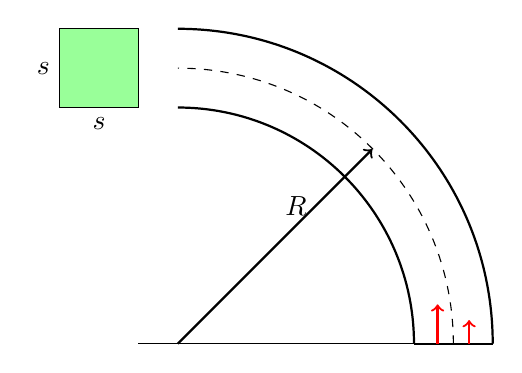
\begin{tikzpicture}
  \filldraw[fill=green!40!white] (-1.5,3) rectangle (-0.5,4);
  \draw[thin] (-0.5,0) -- (3,0);
  \draw[thick,->] (0,0) -- (2.47,2.47);
  \draw[thick] (3,0) -- (4,0);
  %\draw[thick] (0,3) -- (0,4);  
  \draw[thick] (30mm,0mm) arc [start angle=0, end angle=90, radius=30mm];
  \draw[dashed] (35mm,0mm) arc [start angle=0, end angle=90, radius=35mm];  
  \draw[thick] (40mm,0mm) arc [start angle=0, end angle=90, radius=40mm]; 
  \draw (1.5,1.5) node[anchor=south] {$R$};
  \draw (-1,3) node[anchor=north] {$s$};
  \draw (-1.5,3.5) node[anchor=east] {$s$};
  \draw[red,thick,->] (3.3,0) -- (3.3,0.5);%two red arrow
  \draw[red,thick,->] (3.7,0) -- (3.7,0.3);  
  \end{tikzpicture}
%\end{document}
 \caption{圆环通道}\label{fig:52C}
 \end{figure}
 
 由体积流量的定义有
 \begin{align}
 Q=&\int_{0}^s dz \int_{R-\frac{s}{2}}^{R+\frac{s}{2}} v_{\theta} dr\\
 =& As\ln\frac{R+\frac{s}{2}}{R-\frac{s}{2}}\label{eq:52Cap}
 \end{align}
 由式\eqref{eq:52Radius}得
  \begin{equation}
  \rho(-\frac{v^2_{\theta}}{r})=-\frac{\partial p}{\partial r}
 \end{equation}
 沿径向积分得:
  \begin{equation}
  \Delta p=\frac{\rho A^2}{2} \left(\frac{1}{(R-\frac{s}{2})^2}-\frac{1}{(R+\frac{s}{2})^2}\right)
 \end{equation}
 由上式解出$A$代入式\eqref{eq:52Cap}即可。
\section{第六周第一次课}

运用微元控制体推导流体动力学微分型方程的一个例子:

使用柱坐标系下的微元控制体推导连续性方程,如图\ref{fig:61D}
\begin{figure}[!ht]
 \centering
 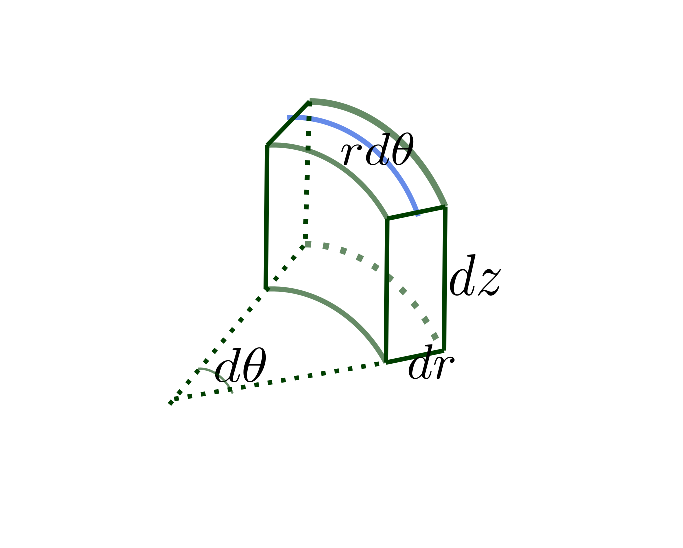
\includegraphics[width=5cm]{differentialControlElement.eps}
 \caption{柱坐标微元控制体}\label{fig:61D}
\end{figure}

对于该微元质量体,$\Delta t$时间内质量变化为
\begin{equation}\label{eq:61cm}
\Delta m = \frac{\partial}{\partial t}(\rho (rd\theta) dr dz)\Delta t
\end{equation}
分别考虑微元质量体六个面的流量,$drdz$确定的两个面分别是左面(可见)与右面。

左面$\Delta t$时间流入量:

\begin{align}\notag
Q_l= & \rho(v_{\theta-\frac{d\theta}{2}}drdz)\Delta t \\
=& (\rho v_{\theta}drdz-\frac{\partial}{\partial \theta}(\rho v_{\theta} drdz)\frac{d\theta}{2})\Delta t
\end{align}
同理得微元体右面$\Delta t$时间流出量
\begin{equation}
Q_r=  (\rho v_{\theta}drdz+\frac{\partial}{\partial \theta}(\rho v_{\theta} drdz)\frac{d\theta}{2})\Delta t \\
\end{equation}
因此微元体左右两个面的净流出量为:
\begin{equation}\label{eq:61crl}
Q_r-Q_l= \frac{\partial}{\partial \theta}(\rho v_{\theta} drdz)d\theta\Delta t
\end{equation}
微元体$rd\theta,dz$确定的前面(可见)和后面的净流出量为:
\begin{align}\notag
Q_b-Q_f =& \rho(v_{r+\frac{dr}{2}}(r+\frac{dr}{2})d\theta dz)\Delta t-\rho(v_{r-\frac{dr}{2}}(r-\frac{dr}{2})d\theta dz)\Delta t\\
=& \frac{\partial }{\partial r}(\rho v_r r d\theta dz)\Delta t\label{eq:61cbf}
\end{align}
同理微元体$rd\theta,dr$确定的上面(可见)和下面的净流出量为:
\begin{equation}\label{eq:61cud}
Q_u-Q_d= \frac{\partial }{\partial z}(\rho v_r rd\theta dr)\Delta t
\end{equation}
根据微元控制体质量守恒,可以得到:
\begin{equation}
-\Delta m=(Q_r-Q_l)+(Q_b-Q_f)+(Q_u-Q_d)
\end{equation}
代入(\ref{eq:61cm},\ref{eq:61crl},\ref{eq:61cbf},\ref{eq:61cud})四个式子得
\begin{align}\notag
-\frac{\partial }{\partial t}(\rho r)=&\frac{\partial }{\partial \theta}(\rho v_{\theta})+
\frac{\partial }{\partial r}(\rho v_r r)+\frac{\partial }{\partial z}(\rho v_z r)\\
\iff & \frac{\partial \rho}{\partial t}+\frac{1}{r}\frac{\partial (\rho v_{\theta})}{\partial \theta}+
\frac{\partial (\rho v_r)}{\partial r}+\frac{\rho v_r}{r}+\frac{\partial(\rho v_z) }{\partial z}=0\label{eq:61cce}
\end{align}
\eqref{eq:61cce}式也可直接从\eqref{eq:52Conti}中利用$\nabla$算子的柱坐标的表达式\eqref{eq:52nablacy}式直接求出。

流体的静力学考虑$\v{v}=\v{0}$,由于流体静止,应变率为零,
因此应力张量$T_{ij}=-p\delta_{ij}$,由\eqref{eq:52Momen}式可以得到流体的静力平衡方程为:
\begin{equation}\label{eq:61static}
\nabla p = \rho \v{f}
\end{equation}
上式两边求旋度得到\eqref{eq:61static}式成立的必要条件:
\begin{equation}\label{eq:61staticNecess}
\nabla \times (\rho \v{f})=\v{0}
\end{equation}
\newglossaryentry{barotropic}
{
  name=正压流体,
  description={$\rho=\rho(p)$,即密度只与压力有关}
}
若\glsdesc{barotropic},那么称流体为\gls{barotropic},对于正压流体,定义压力函数
$\mathbb{P}$为:
\begin{equation}
\mathbb{P}=\int \frac{1}{\rho(p)}dp
\end{equation}
则容易求出压力函数$\mathbb{P}$的梯度为
\begin{equation}\label{eq:61barotropicPotential}
\nabla \mathbb{P} =\frac{d \mathbb{P}}{dp} \nabla p = \frac{\nabla p}{\rho}
\end{equation}
即对于正压流体,$\frac{\nabla p}{\rho}$有势。

在这种情况下$\nabla \rho=\frac{d\rho}{dp}\nabla p$,
因此\eqref{eq:61staticNecess}式化简为:
\begin{align}
&\nabla \rho \times \v{f} + \rho \nabla \times \v{f} =  \v{0}\label{eq:61staticExpand}\\
\Rightarrow & \frac{d\rho}{dp}\nabla p \times \frac{\nabla p}{\rho} + \rho \nabla \times \v{f} =  \v{0}\nonumber\\
\Rightarrow  &  \nabla \times \v{f} =  \v{0}\label{eq:61barotropic}
\end{align}
即对于处于静止状态的正压流体,体积力是有势场。
我们可以说明\eqref{eq:61barotropic}式也是正压流体的充分条件,即在静力平衡方程的基础上,如果有\eqref{eq:61barotropic}式
成立,那么$\rho$与$p$存在单值映射关系。
\begin{align}
&\nabla \times \v{f} =  \v{0}\nonumber\\
\Rightarrow & \nabla \times \frac{\nabla p}{\rho} =  \v{0}\nonumber\\
\Rightarrow  &   \nabla \frac{1}{\rho} \times \nabla p =  \v{0}\label{eq:61parallel}
\end{align}
由\eqref{eq:61parallel}可得到关于$\nabla \frac{1}{\rho}$各阶分量的一阶PDE,附加适当的边界条件可以得到$\frac{1}{\rho}$关于
$\nabla p$和边界条件的解。因此$\frac{1}{\rho}$与$p$的地位在\eqref{eq:61parallel}式是对等的,所以我们可以得到$\rho$与$p$存在单值映射关系。

对于一般的情形,若流体静止,对\eqref{eq:61staticExpand}式两边点乘$\v{f}$,\eqref{eq:61staticExpand}式左边第一项得零,因此我们得到
流体静止体积力的一个必要条件为
\begin{equation}
\v{f}\cdot (\nabla \times \v{f})=0
\end{equation}
若外力场是重力场,$\v{f}=-g\v{k}$,对于密度为常量的液体,可以得到
\begin{equation}
p=-\rho g z + p_{z=0}
\end{equation}
如果我们考虑一具有恒定水平加速度$\v{a}=a\v{i}$的非惯性系,并且取坐标原点在自由液面上,则
\begin{equation}
p=-\rho(gz+ax)+p_a
\end{equation}
$p_a$代表大气压,同时由上式可以得到自由液面的形状在惯性系中具有$gz+ax=0$这种倾斜的直线的形状。
\section{第六周第二次课}

理想流体运动的基本方程
理想流体应力张量$T_{ij}=-p\delta_{ij}$,因此动量方程\eqref{eq:52Momen}式化为:
\begin{equation}\label{eq:62EulerEq}
 \frac{\partial \v{v}}{\partial t}+\v{v}\cdot\nabla\v{v}=\v{f}-\frac{1}{\rho}\nabla\cdot p
\end{equation}
\eqref{eq:62EulerEq}式即欧拉方程,
相应的\eqref{eq:52Energy}化为
\begin{equation}\label{eq:62IdealEnergy}
 \frac{D(e+\frac{1}{2}|\v{v}|^2)}{Dt}=
 \v{f}\cdot\v{v}-\frac{1}{\rho}\nabla\cdot(p\v{v})+(\dot{q}+q_R) 
\end{equation}

综合连续性方程\eqref{eq:52Conti}式,\eqref{eq:62EulerEq},\eqref{eq:52Energy}
共5个方程,但未知数有$\v{v},e,p,\rho\,$ 6个,因此需补充热力学方程才能使方程组封闭。

实际上,我们可以通过动量方程\eqref{eq:62EulerEq}式得到动能的变化率:
\begin{equation}\label{eq:62KinematicEneryChangeRate}
\frac{D}{D t}(\frac{1}{2}|\v{v}|^2)=\v{f}\cdot \v{v}-\frac{1}{\rho}\v{v}\cdot\nabla p
\end{equation}
将\eqref{eq:62IdealEnergy}式与\eqref{eq:62KinematicEneryChangeRate}作差得:
\begin{align}
\frac{De}{Dt}= & -\frac{p}{\rho} \nabla \cdot \v{v} + \dot{q}+q_R ,\text{by }\eqref{eq:52ContiMaterial}\nonumber\\
=& \frac{p}{\rho^2}\frac{D\rho}{Dt} + \dot{q}+q_R \nonumber\\
=& -p\frac{D}{Dt}\left(\frac{1}{\rho}\right) + \dot{q}+q_R\label{eq:62DeDt1}
\end{align}
定义$i=e+\frac{p}{\rho}$为气体的焓,则可以得到
\begin{equation}
\frac{D i}{D t}=\dot{q}+q_R + \frac{1}{\rho} \frac{D p }{D t}
\end{equation}
对于绝热状态下的理想常比热完全气体,我们有
\begin{align}
\frac{D e}{D t}=& C_V \frac{D T}{D t},e=C_V T\nonumber\\
=& \frac{C_V}{R} \frac{D}{D t}\left(\frac{p}{\rho}\right),p=\rho RT\nonumber\\
=& \frac{1}{\gamma -1} \frac{D}{D t}\left(\frac{p}{\rho}\right),C_P-C_V=R,\frac{C_P}{C_V}=\gamma \label{eq:62DeDt2}
\end{align}
将\eqref{eq:62DeDt1}式去掉产热项,与\eqref{eq:62DeDt2}式结合可以得到
\begin{equation}\label{eq:62prho}
\frac{D}{D t}\left(\frac{p}{\rho^{\gamma}}\right)=0
\end{equation}
\eqref{eq:62prho}式即为对于气体补充的$\rho$和$p$的关系的热力学方程。

对于匀质不可压缩的液体,补充$\nabla \cdot \v{v}=0$的方程,此时\eqref{eq:52Conti}式恒成立,动力学方程与热力学方程解耦,
因此我们可以联立求解:
\begin{align}\notag
\nabla \cdot \v{v}=&0\\
 \frac{\partial \v{v}}{\partial t}+\v{v}\cdot\nabla\v{v} =&\v{f}-\frac{1}{\rho}\nabla\cdot p
\end{align}
得到$\v{v},p$再代入能量方程求其他参量。

下面考虑理想流体动力学偏微分方程的边界条件。一般的,对于不可穿透的壁面,流体的法向速度与壁面运动的法向速度相等,即满足:
\begin{equation}
(\v{v}_L\cdot \v{n})_{\Sigma}=(\v{v}_B\cdot \v{n})_{\Sigma}
\end{equation}
若$\Sigma$有曲面方程$F(x,y,z,t)=0$,则流体边界速度满足
\begin{equation}
\frac{\partial F}{\partial t} + \v{v_L} \cdot \nabla F=0
\end{equation}
此即\textbf{不可穿透条件}的一种提法;此外,我们还有无穷远条件等。

\begin{equation}
\end{equation}

对于球坐标,基矢量随坐标变量的变化规律为\cite{Del}:
\begin{align}
\frac{\partial \v{e_r}}{\partial \theta}=&\v{e_{\theta}},\,\,  \frac{\partial \v{e_r}}{\partial \varphi}=\v{e_{\varphi}}\sin\theta\\
\frac{\partial \v{e_{\theta}}}{\partial \theta}=&-\v{e_r},\,\,  \frac{\partial \v{e_{\theta}}}{\partial \varphi}=\v{e_{\varphi}}\cos\theta\\
\frac{\partial \v{e_{\varphi}}}{\partial \varphi}=&-(\v{e_r}\sin\theta+\v{e_{\theta}}\cos\theta)
\end{align}

球坐标系下的梯度算子表示为:
\begin{equation}
\nabla = \frac{\partial }{\partial r} \v{e_r} + \frac{1}{r} \frac{\partial}{\partial \theta} \v{e_{\theta}}+
\frac{1}{r\sin\theta}
\frac{\partial }{\partial \varphi}\v{e_{\varphi}}
\end{equation}

因此球坐标系下对于矢量$\v{v}=v_r\v{e_r}+v_{\theta}\v{e_{\theta}}+v_{\varphi}\v{e_{\varphi}}$的散度为:
\begin{align*}
&(\frac{\partial }{\partial r} \v{e_r} + \frac{1}{r} \frac{\partial}{\partial \theta} \v{e_{\theta}}+\frac{1}{r\sin\theta}
\frac{\partial }{\partial \varphi}\v{e_{\varphi}})\cdot (v_r\v{e_r}+v_{\theta}\v{e_{\theta}}+v_{\varphi}\v{e_{\varphi}}) =\\
&\frac{\partial v_r}{\partial r}+\frac{1}{r}\frac{\partial v_{\theta}}{\partial \theta}+\frac{1}{r\sin\theta}
\frac{\partial v_{\varphi}}{\partial \varphi} +\frac{v_r}{r}\frac{\partial \v{e_r}}{\partial \theta}\cdot \v{e_{\theta}}+
(v_r\frac{\partial \v{e_r}}{\partial \varphi}+v_{\theta}\frac{\partial \v{e_{\theta}}}{\partial \varphi}+
v_{\varphi}\frac{\partial \v{e_{\varphi}}}{\partial \varphi})\cdot \frac{\v{e_{\varphi}}}{r \sin\theta}\\
=&\frac{\partial v_r}{\partial r}+\frac{1}{r}\frac{\partial v_{\theta}}{\partial \theta}+\frac{1}{r\sin\theta}
\frac{\partial v_{\varphi}}{\partial \varphi} +\frac{v_r}{r}+
(v_r\sin\theta+v_{\theta}\cos\theta)\frac{1}{r \sin\theta}\\
=&\frac{\partial v_r}{\partial r}+\frac{1}{r}\frac{\partial v_{\theta}}{\partial \theta}+\frac{1}{r\sin\theta}
\frac{\partial v_{\varphi}}{\partial \varphi} +\frac{2v_r}{r}+\frac{v_{\theta}\cos\theta}{r \sin\theta}
\end{align*}
所以
\begin{equation}
\nabla \cdot \v{v}=\frac{1}{r^2}\frac{\partial (r^2 v_r)}{\partial r}+
\frac{1}{r\sin\theta}\frac{\partial (v_{\theta}\sin\theta)}{\partial \theta}+
\frac{1}{r\sin\theta}\frac{\partial v_{\varphi}}{\partial \varphi} 
\end{equation}
\begin{equation}
\end{equation}

\section{第七周第一次课}
涡量方程:
\eqref{eq:52NSEqUnCompress}式给出了不可压流的N-S方程,对于一般情形,在\eqref{eq:52TijUn}式中代入\eqref{eq:52TSG}式(取$\mu'=0$)于是有
\begin{align}
\nabla\cdot \bm{T} = & -\nabla p+\mu \nabla^2 \v{v} +\mu \frac{\partial^2 v_i}{\partial x_i \partial x_j} \v{e}_j + \frac{\partial }{\partial x_i} (-\frac{2}{3}\mu \nabla\cdot \v{v}\delta_{ij})\v{e}_j, \text{eq\eqref{eq:52nablav0C} invalid}\\
= & -\nabla p+\mu \nabla^2 \v{v} + \frac{\mu}{3}\nabla(\nabla \cdot \v{v})
\end{align}
因此我们得到一般形式的N-S方程:
\begin{equation}\label{eq:71generalNS}
\frac{\partial \v{v}}{\partial t}+\v{v}\cdot\nabla\v{v}=\v{f}-\frac{\nabla p}{\rho}+\frac{\mu}{\rho} (\frac{1}{3}\nabla(\nabla\cdot \v{v})+\nabla^2 \v{v})
\end{equation}

通过对上式两边取旋度可以得到涡量方程,为此,首先推导:
\begin{equation}\label{eq:71vvw}
2\v{v}\cdot \nabla \v{v}=\nabla (\v{v}\cdot\v{v}) + 2(\nabla\times \v{v})\times \v{v} 
\end{equation}

\begin{align*}
\text{RHS}=& \frac{\partial v_i^2}{\partial x_j} \v{e_j} + 2(\epsilon_{ijk}\frac{\partial v_k}{\partial x_j}\v{e_i})\times \v{v}\\
=& \frac{\partial v_i^2}{\partial x_j} \v{e_j} + 2(\epsilon_{min}\epsilon_{ijk}\frac{\partial v_k}{\partial x_j}v_n)\v{e_m}\\
=& 2v_i\frac{\partial v_i}{\partial x_j} \v{e_j} - 2((\delta_{mj}\delta_{nk}-\delta_{mk}\delta_{nj})\frac{\partial v_k}{\partial x_j}v_n)\v{e_m}\\
=& 2v_i\frac{\partial v_i}{\partial x_j} \v{e_j} - 2(\frac{\partial v_k}{\partial x_j}v_k)\v{e_j}+2(\frac{\partial v_k}{\partial x_j}v_j)\v{e_k}\\
=& 2(\frac{\partial v_k}{\partial x_j}v_j)\v{e_k}\\
= \text{LHS}
\end{align*}

再推导
\begin{equation}
\nabla\times(\v{A}\times \v{B})=(\nabla\cdot \v{B}+\v{B}\cdot\nabla)\v{A}-(\nabla\cdot \v{A}+\v{A}\cdot\nabla)\v{B}
\end{equation}

\begin{align*}
\text{LHS}=&\nabla\times(\epsilon_{ijk}A_jB_k\v{e_i})\\
=& \epsilon_{mni}\epsilon_{ijk}\frac{\partial (A_jB_k)}{\partial x_n}\v{e_m}\\
=& (\delta_{mj}\delta_{nk}-\delta_{mk}\delta_{nj})(B_k\frac{\partial A_j}{\partial x_n}+A_j\frac{\partial B_k}{\partial x_n})\v{e_m}\\
=&(B_k\frac{\partial A_j}{\partial x_k}+A_j\frac{\partial B_k}{\partial x_k})\v{e_j}
-(B_k\frac{\partial A_j}{\partial x_j}+A_j\frac{\partial B_k}{\partial x_j})\v{e_k}\\
=& \text{RHS}
\end{align*}

因此,由\eqref{eq:71generalNS}式我们有:
\begin{align*}
\nabla\times \text{LHS}=& \nabla\times (\frac{\partial \v{v}}{\partial t}+\v{v}\cdot\nabla\v{v})\\
=& \frac{\partial }{\partial t}(\nabla\times \v{v})+\nabla\times(\v{v}\cdot\nabla\v{v}) \\
=& \frac{\partial \v{w}}{\partial t}+\nabla\times(\nabla \frac{|\v{v}|^2}{2}+\v{w}\times \v{v})\\
=& \frac{\partial \v{w}}{\partial t} +(\nabla\cdot\v{v})\v{w}-(\nabla\cdot\v{w})\v{v}
+(\v{v}\cdot\nabla)\v{w}-(\v{w}\cdot\nabla)\v{v},\nabla\cdot\v{w}=0 \\
=& \frac{D \v{w}}{D t} +(\nabla \cdot \v{v})\v{w}-(\v{w}\cdot\nabla)\v{v}
\end{align*}

而上式右端:
\begin{align*}
\nabla\times \text{LHS}=& \nabla\times\left(\v{f}-\frac{\nabla p}{\rho}+\frac{\mu}{\rho} (\frac{1}{3}\nabla(\nabla\cdot \v{v})+\nabla^2 \v{v})\right)\\
=& \nabla\times \v{f}-\nabla\frac{1}{\rho}\times \nabla p + \frac{\mu}{\rho}\nabla\times \nabla^2\v{v}+\nabla\left(\frac{\mu}{\rho}\right)\times(\frac{1}{3}\nabla(\nabla\cdot \v{v})+\nabla^2 \v{v})
\end{align*}
因此我们由不可压的N-S方程得到了涡量方程的一般形式:
\begin{equation}
\frac{D \v{w}}{D t} +(\nabla \cdot \v{v})\v{w}-(\v{w}\cdot\nabla)\v{v}=\nabla\times \v{f}-\nabla\frac{1}{\rho}\times \nabla p + \frac{\mu}{\rho}\nabla\times \nabla^2\v{v}+\nabla\left(\frac{\mu}{\rho}\right)\times(\frac{1}{3}\nabla(\nabla\cdot \v{v})+\nabla^2 \v{v})
\end{equation}
从上面的涡量方程可以看出,对于理想正压流体,若质量力有势,方程右端项为零。
由连续性方程\eqref{eq:52ContiMaterial}式左端可化简为
\begin{equation}
\frac{1}{\rho}\frac{D\v{w}}{Dt}+\frac{D}{Dt}\left(\frac{1}{\rho}\right) \v{w}-\left(\frac{\v{w}}{\rho}\right)\cdot \nabla \v{v}=0
\end{equation}
即整理为
\begin{equation}
\frac{D}{Dt}\left(\frac{\v{w}}{\rho}\right)=\left(\frac{\v{w}}{\rho}\right)\cdot\nabla\v{v}
\end{equation}
%如何说明 Lagrange 定理??

% 下面以信风的形成为例说明非正压流场速度环量非零。

% \begin{figure}[!ht]
 % \centering
 % %LaTeX with PSTricks extensions
%%Creator: inkscape 0.92.2
%%Please note this file requires PSTricks extensions
%\documentclass{article}
%\pagestyle{empty}
%\usepackage{tikz}
%\begin{document}
 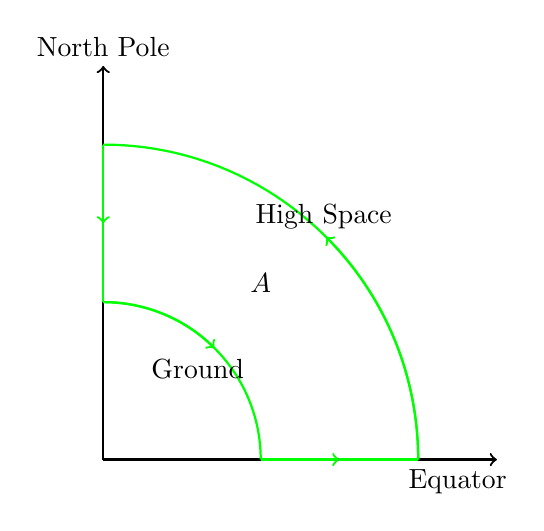
\begin{tikzpicture}
  \draw[thick,->] (0,0) -- (5,0);
  \draw[thick,->] (0,0) -- (0,5);
  \draw[thick,green,->] (2,0) -- (3,0);
  \draw[thick,green] (3,0) -- (4,0);  
  \draw[thick,green] (0,2) -- (0,3);
  \draw[thick,green,->] (0,4) -- (0,3);    
  \draw[thick,green] (2,0) arc [start angle=0, end angle=90, radius=2]; %ground
  \draw[thick,green,->] (0,2) arc [start angle=90, end angle=45, radius=2]; %ground
  \draw[thick,green] (4,0) arc [start angle=0, end angle=90, radius=4]; %high space
  \draw[thick,green,->] (4,0) arc [start angle=0, end angle=45, radius=4]; %high space
  \draw (4.5,0) node[anchor=north] {Equator};  
  \draw (0,5) node[anchor=south] {North Pole};      
  \draw (1.2,1.4) node[anchor=north] {Ground};      
  \draw (2.8,2.8) node[anchor=south] {High Space};        
  \draw (2,2) node[anchor=south] {$A$};  
  \end{tikzpicture}
%\end{document}

 % \caption{信风风向示意图}\label{fig:71tradeWind}
% \end{figure}

% 由图\ref{fig:71tradeWind}可以看出,在近地面,风向主要是由北极到赤道附近,在高空风向相反。这种风向可以通过
% 判断速度环量的正负确定,假设大气是理想流体,则有
% \begin{align*}
% \frac{D}{Dt}\oint_l \v{v}\cdot\v{x} =& - \oint_l \frac{\nabla p}{\rho}\cdot\v{x}\\
% = & \iint_{A} \frac{1}{\rho^2}(\nabla \rho \times \nabla p )\cdot\v{n}dA
% \end{align*}
% 在同一条等压线上,由于赤道与北极温度不同,由理想气体状态方程可知密度不同,因此等压线与等密度线不重合,$\nabla \rho \times \nabla p \neq \v{0}$
% 为更细致的判断上式的符号,我们考虑一个理想的场景。


% 对于非有势力场,速度环量一般也不为零,下面以地转偏向力的形成为例说明:
% \begin{figure}[!ht]
 % \centering
 % 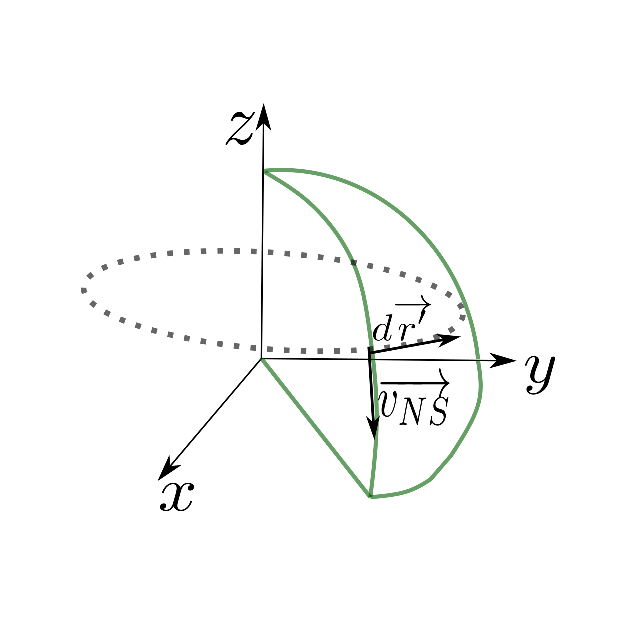
\includegraphics[width=5cm]{Coriolis_Force.eps}
 % \caption{北半球流线偏转示意图}\label{fig:71NorthStreamLine}
% \end{figure}

% 如图\ref{fig:71NorthStreamLine}所示,考虑一不与纬线平行的流线,其相对地球坐标系的涡量变化为(假设为正压流体):
% \begin{equation}
% \frac{D \Gamma'}{D t}=\oint_l -\v{a} \cdot d\v{r'}
% \end{equation}
% 对于转动坐标系中的加速度,有
% \begin{equation}\label{eq:71accelerate}
% \v{a}=\v{\omega}\times(\v{\omega}\times\v{R'})+2\v{\omega}\times\v{v'}
% \end{equation}
% 第一项为向心加速度,与$\v{r'}$垂直,对于第二项,只有在南北向的相对速度分量(球坐标系中为$\v{e_{\theta}}$方向)起作用,
% 因此$(\v{\omega}\times\v{v_{NS}})\cdot d\v{r'} =\v{\omega}\cdot(\v{v_{NS}}\times d\v{r'})$
% Physical Meaning Of Velocity Circuit?
% \begin{equation}
% \end{equation}

Lamb 型方程:考虑对理想气体,由欧拉方程\eqref{eq:62EulerEq}式和\eqref{eq:71vvw}式得到
\begin{equation}\label{eq:71Lamb}
 \frac{\partial \v{v}}{\partial t}+\nabla(\frac{1}{2}|\v{v}|^2)-\v{v}\times \v{\Omega}=\v{f}-\frac{1}{\rho}\nabla\cdot p
\end{equation}
其中$\v{v}\times \Omega$被称为Lamb矢量,若考虑质量力有势的正压定常流体,上式沿流线或涡线积分即可得到Bernoulli守恒方程:
\begin{equation}
\int_l \v{s}\cdot (\nabla(\frac{1}{2}|\v{v}|^2)-\v{v}\times \v{\Omega})ds=\int_l \v{s}\cdot (-\nabla\Pi-\nabla \mathbb{P})ds
\end{equation}
注意到$\v{s}$与$\v{v}$或$\v{\Omega}$平行,因此$\v{s}\cdot(\v{v}\times \v{\Omega})=0$,于是得到
\begin{equation}\label{eq:71LambBernoulli}
\frac{1}{2}v^2+\mathbb{P}+\Pi=C
\end{equation}
针对\eqref{eq:71Lamb}式,如考虑用常比热完全气体的等熵过程($\frac{p}{\rho^{\gamma}}=c$)代替正压的条件,则压力势项可改写为
\begin{align*}
\mathbb{P}=&\int \frac{dp}{\rho}\\
=& \int c\frac{d\rho^{\gamma}}{\rho}\\
=& \int c \gamma d \rho^{\gamma-2} d\rho\\
=& \int c \frac{\gamma}{\gamma-1} \rho^{\gamma-1}\\
=& \frac{\gamma}{\gamma-1}\frac{p}{\rho}
\end{align*}
因此对常比热完全气体的等熵过程,Bernoulli方程为
\begin{equation}
\frac{1}{2}v^2+\frac{\gamma}{\gamma-1}\frac{p}{\rho}+\Pi=C
\end{equation}
同理可推出对完全气体的等温过程
\begin{equation}
\frac{1}{2}v^2+RT\ln p+\Pi=C
\end{equation}
下面考虑流体相对等转速坐标系$O'x'y'$下的Bernoulli方程,转动坐标系相对静止坐标系的关系如下图所示:
\begin{figure}[!ht]
 \centering
 %LaTeX with PSTricks extensions
%%Creator: inkscape 0.92.2
%%Please note this file requires PSTricks extensions
%\documentclass{article}
%\pagestyle{empty}
%\usepackage{tikz}
%\begin{document}
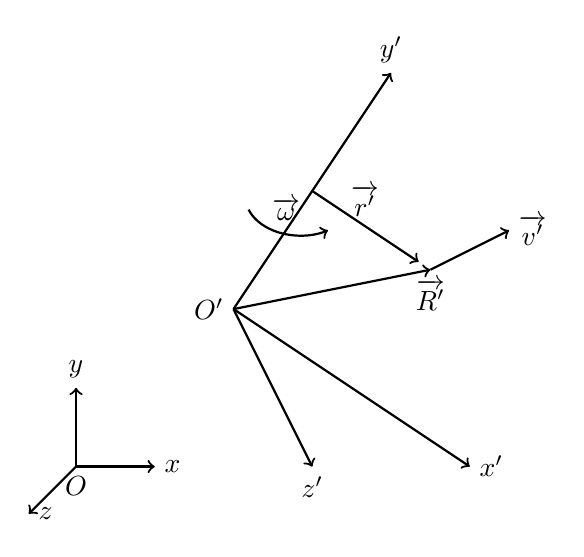
\begin{tikzpicture}
%reference coordinate 
  \draw[thick,->] (0,0) -- (1,0);
  \draw[thick,->] (0,0) -- (0,1);
  \draw[thick,->] (0,0) -- (-0.6,-0.6);  
  \draw (0,0) node[anchor=north] {$O$};  
  \draw (1,0) node[anchor=west] {$x$};      
  \draw (0,1) node[anchor=south] {$y$};      
  \draw (-0.6,-0.6) node[anchor=west] {$z$};      
  %rotational coordinate
  \draw[thick,->] (2,2) -- (5,0);
  \draw[thick,->] (2,2) -- (4,5);    
  \draw[thick,->] (2,2) -- (3,0);      
  \draw (2,2) node[anchor=east] {$O'$};  
  \draw (5,0) node[anchor=west] {$x'$};      
  \draw (4,5) node[anchor=south] {$y'$};      
  \draw (3,0) node[anchor=north] {$z'$};        
%point interested
  \draw[thick,->] (2,2) -- (4.5,2.5);%R'
  \draw[thick,->] (4.5,2.5) -- (5.5,3);%v'  
  \draw (4.5,2.5) node[anchor=north] {$\v{R'}$};    
  \draw (5.5,3) node[anchor=west] {$\v{v'}$};      
  \draw[thick,->] (3,3.5) -- (4.35,2.6);%r'
  \draw (3.67,3.05) node[anchor=south] {$\v{r'}$};
  \draw (2.67,3) node[anchor=south] {$\v{\omega}$};  
  \draw[thick,<-] (3.2,3) arc [start angle=300, end angle=200, x radius=0.7, y radius=0.5];
  \end{tikzpicture}
%\end{document}

 \caption{等转速坐标系下的Bernoulli方程推导示意}\label{fig:71rotationalCoordinateBernoulli}
\end{figure}
这里,我们去掉正压流体的假设,而附加绝热条件,于是\eqref{eq:62Enthalpy}式焓的随体导数可简化为:
\begin{align*}
\frac{D i}{D t} = &\frac{1}{\rho} \frac{D p}{D t}\\
\Rightarrow  \v{v}\cdot \nabla i =& \frac{1}{\rho} \v{v}\cdot \nabla p
\end{align*}
最后一式用到了定常流的条件,由于$\v{v}$的任意性,所以$\nabla i = \frac{\nabla p}{\rho}$,即
$\frac{\nabla p}{\rho}$有势函数$i$。

从\eqref{eq:71Lamb}式出发,由于是在转动坐标系中,我们对$\v{f}$有加速加项的修正,即以$\v{f}-\v{a}$
代替\eqref{eq:71Lamb}式中的$\v{f}$。$\v{a}$的表达式由\eqref{eq:71accelerate}式给出
\begin{equation}\label{eq:71accelerate}
\v{a}=\v{\omega}\times(\v{\omega}\times\v{R'})+2\v{\omega}\times\v{v'}
\end{equation}

注意到$\v{a}$的第二项$\v{v'}$含$\v{v'}$,如沿相对流线积分,同样由$\v{s'}$与$\v{v'}$平行的性质得其积分为零,因此,只需考虑
$\v{a}$的第一项
\begin{equation}\label{eq:71MiddleResultOmega}
\v{\omega}\times(\v{\omega}\times\v{R'}) = (\v{\omega}\cdot \v{R'})\v{\omega}-(\v{\omega}\cdot \v{\omega})\v{R'}
\end{equation}
我们这里设$\v{\omega}$沿$y'$轴,即$\v{\omega}=\omega \v{e_{y'}}$,
考虑$(\v{\omega}\cdot \v{\omega})\v{R'}$在$\v{e_{y'}}$方向的投影为$\omega^2(\v{R'}\cdot \v{e_{y'}})$,而
$(\v{\omega}\cdot \v{R'})\v{\omega}=\omega^2(\v{R'}\cdot \v{e_{y'}})\v{e_{y'}}$,因此\eqref{eq:71MiddleResultOmega}式可化简为
$(\v{\omega}\cdot \v{\omega})\v{R'}$在$O'x'z'$平面上的投影长度的相反数:
%\begin{align*}
%\end{align*}
\begin{equation}
\v{\omega}\times(\v{\omega}\times\v{R'})=-\omega^2 \v{r'}
\end{equation}
其中$\v{r'}$为$\v{R'}$在$Ox'z'$平面上的投影向量,并假设转动角速度$\omega$为常数,则
\begin{equation}
\v{\omega}\times(\v{\omega}\times\v{R'})=-\nabla' (\frac{1}{2}\omega^2 r'^2)
\end{equation}
这里$\nabla'$表示相对转运坐标系的梯度算子,所以$\v{a}$项在沿相对流线积分得到$\frac{1}{2}\omega^2 r'^2$。
综合上面的结果,我们得到等转速坐标系下的Bernoulli方程为:
\begin{equation}
\frac{1}{2}v'^2+\Pi+i-\frac{1}{2}\omega^2 r'^2 = c
\end{equation}
\begin{equation}
\end{equation}
\begin{equation}
\end{equation}

\section{第七周第二次课}
上节我们从Lamb型方程\eqref{eq:71Lamb}式出发推导了Bernoulli方程的各种变形,如果我们去掉定常流的条件而附加流场无旋的条件,
那么\eqref{eq:71Lamb}式中Lamb矢量为零,由于流体无旋,存在速度势函数$\varphi$,使得$\v{v}=\nabla \varphi$。
积分\eqref{eq:71Lamb}式得到Cauchy-Lagrange 积分方程(CL方程):
\begin{equation}\label{eq:72CLEquation}
\frac{\partial \varphi}{\partial t}+\frac{1}{2} |\nabla \varphi|^2+\mathbb{P}+\Pi=C(t)
\end{equation}

下面是一个应用CL方程的一个例子:

考虑一个长为$2l$的L型两端开口直管,下端封闭,上端与大气接触,里面充满理想均质不可压的液体,如图(\ref{fig:72CL_integral_example}.a)所示:
\begin{figure}[!ht]
 \centering
 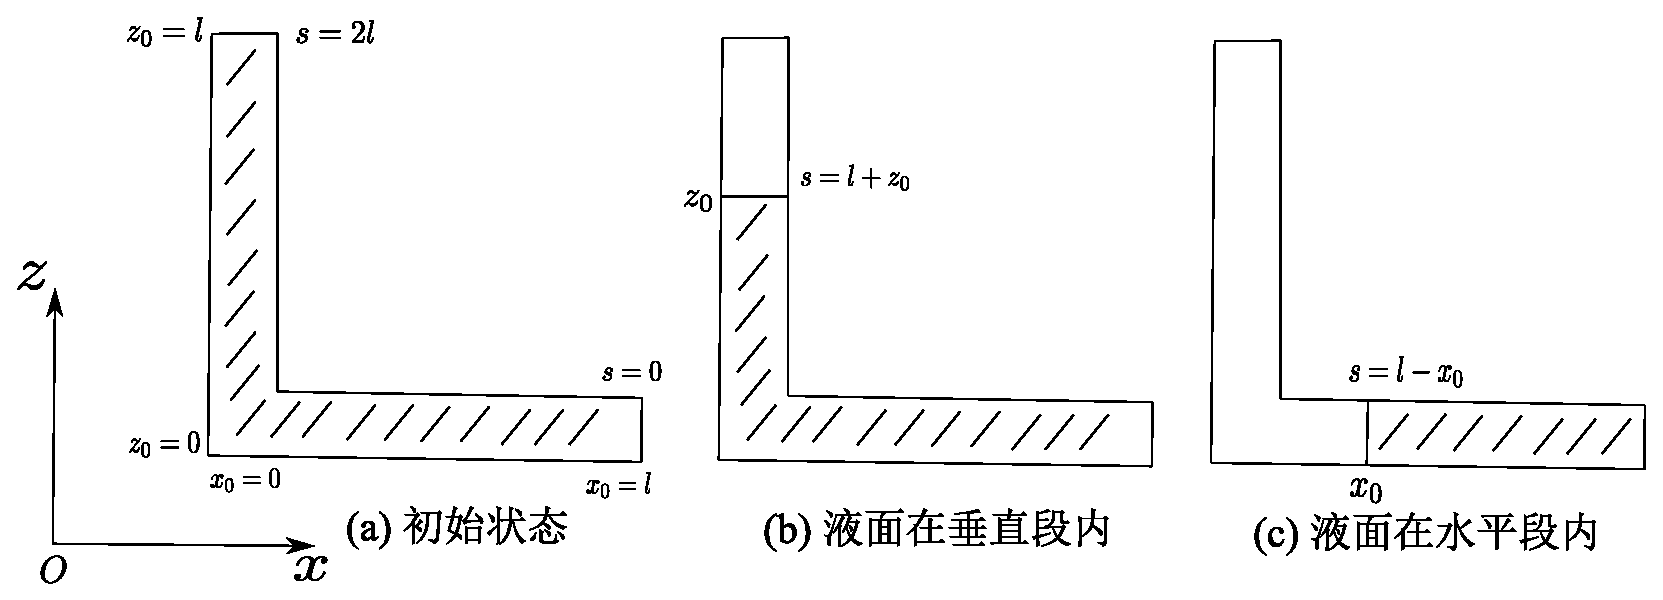
\includegraphics[width=9cm]{CL_integral_example.eps}
 \caption{L型直管}\label{fig:72CL_integral_example}
\end{figure}

当释放直管的下端使液体流出时,
管内压强和出口处的速度会发生突变。我们先来求出口处的速度。为此,取类似于弧长坐标系的一维局部坐标$s$表示离出口处的液柱长度为
$s,0\leq s\leq 2l$,则$\v{v}(t)=-v\v{e_s}$,因为流体不可压,所以$\frac{\partial v}{\partial s}=0$,即$v=v(t)$,又因为速度场有势,
所以存在势函数$\varphi(s,t)$,使得$\frac{\partial \varphi}{\partial s}=-v(t)$,如取$s=0$时速度势为零,则$\varphi(t,s)=-v(t)s$,
所以 \eqref{eq:72CLEquation}式化为:
\begin{equation}\label{eq:72CLEqExample}
-v'(t)s+\frac{1}{2}v^2(t)+\frac{p}{\rho}+\Pi=C(t)
\end{equation}
当直管的下端释放时,分别考虑$s=0$和$s=2l$两端,$p=p_a$,均为大气压,速度均为$0$,$\Pi(2l)=gl$,由上式求出:
\begin{equation}
v'(0)=\frac{1}{2}g,C(0)=\frac{p_a}{\rho}
\end{equation}
如果考虑任意截面$s$处,则有
\begin{equation}
-v'(0)s+\frac{p}{\rho}+\Pi(s)=\frac{p_a}{\rho}
\end{equation}
于是得任意截面$s$处初始时刻压强的分布为:
\begin{equation}
p(s)=p_a+\frac{1}{2}\rho g s-\rho \Pi(s)
\end{equation}
而$\Pi(s)$可写成分段函数的形式:
\begin{equation}
\Pi(s)=\begin{cases}
g(s-l) & l\leq s\leq 2l\\
0 & 0 \leq s < l
\end{cases}
\end{equation}

下面我们考虑液体完全流出时管口的流速,
由CL方程\eqref{eq:72CLEqExample}式得到液面$s=z_0$处和出口处$s=0$时的平衡方程为
\begin{equation}\label{eq:72SimularNewton}
v'(t) (l+z_0)=\Pi(z_0)
\end{equation}
由于$\Pi$是$f$的分段函数,为此,分两阶段考虑:
当液面在垂直段内时,如图(\ref{fig:72CL_integral_example}.b)所示,此时取$z_0$坐标研究问题比较方便:
设$z_0=z_0(t)$,$z_0$随时间减小,$\Pi(z_0)=gz_0,v=-\frac{d z_0}{dt}$,代入到\eqref{eq:72SimularNewton}式中有:
\begin{equation}
-\frac{d^2 z_0}{dt^2} = \frac{g z_0}{l+z_0}
\end{equation}
上式是标准的 Newton 运动学方程,可用能量方法先求出液面降到$f$时液面处速度
$v_{z_0=f}$为:
\begin{equation}
\frac{1}{2}v_{z_0=f}^2=\int_{f}^{l} \frac{g z_0}{l+z_0} dz_0
\end{equation}
解得:
\begin{equation}
\frac{1}{2}v^2_{z_0=f}=g(l-f)+gl\ln \left(\frac{l+f}{2l}\right)
\end{equation}
由此求得$f=0$时的速度为:$v_{z_0=0}=\sqrt{2gl(1-\ln 2)}$
由$v=-\frac{d z_0}{dt}$上式可化为:
\begin{equation}
-\frac{d z_0}{\sqrt{2g(l-z_0)+2gl\ln(l+f)-2gl\ln(2l)}}=dt
\end{equation}
当$z_0$从$l$到$0$时,时间从$0$到液面$z_0$下降到0的时间$T_1$,因此分别对上式两边积分:
\begin{equation}
\int_0^l \frac{d z_0}{\sqrt{2g(l-z_0)+2gl\ln(l+z_0)-2gl\ln(2l)}}=T_1
\end{equation}
变量替换:
\begin{equation}
T_1=\sqrt{\frac{l}{2g}}\int_0^1 \frac{d z_0}{\sqrt{(1-z_0)+\ln(1+z_0)-\ln 2}}=T_1
\end{equation}
数值积分得:$T_1=2.13\sqrt{\frac{l}{g}}$

当液面在水平段内时,如图(\ref{fig:72CL_integral_example}.c)所示,此时由于$\Pi$不随位置变化,由\eqref{eq:72SimularNewton}式可知
速度也不随时间变化。因此液体将以$v_{z_0=0}$的速度匀速流过长为$l$的水平段,用时$T_2=\frac{l}{v_{z_0=0}}=1.28\sqrt{\frac{l}{g}}$
将$T_1$和$T_2$求和即得到液体全部流出的总的时间。

CL积分方程中若速度势$\phi$用动坐标系下的坐标表示,$\nabla$与坐标表示无关,直接改写为$\nabla'$,
但局部导数项$\frac{\partial}{\partial t}$需做相应变换。
考虑到随体导数与坐标表示无关,即
\begin{equation}
\frac{D\varphi}{Dt}=\frac{D'\varphi}{Dt}
\end{equation}
两边展开得
\begin{equation}
\frac{\partial \varphi}{\partial t}+\nabla \phi \cdot \v{v}=\frac{\partial' \varphi}{\partial t}+\nabla' \phi \cdot \v{v'}
\end{equation}
对于$\nabla \varphi$和$\nabla' \varphi$,均表示绝对速度$\v{v}$,只不过一个在绝对坐标系中表示,一个在相对坐标系中。
而$\v{v'}$表示相对速度而不是绝对速度在动坐标系下的表示。

因此我们得到
\begin{align}\notag
\frac{\partial \varphi}{\partial t}=&\frac{\partial' \varphi}{\partial t}+(\v{v'}-\v{v})\cdot \v{v}\\
=&\frac{\partial' \varphi}{\partial t}-\v{v_e}\cdot \v{v}
\end{align}

从而由\eqref{eq:72CLEquation}式得到速度势在相对坐标系下表示的CL积分方程为:
\begin{equation}\label{eq:72CLRelative}
\frac{\partial' \varphi}{\partial t}-\v{v_e}\cdot \nabla'\varphi+\frac{1}{2} |\nabla'\varphi|^2+\mathbb{P}+\Pi=C(t)
\end{equation}

下面是\eqref{eq:72CLRelative}式应用的一个例子:

一半径为$a$的圆球在无限大的理想正压无旋不可压流体中以$\v{v_o}(t)$的速度做变速直线运动,
求流体表面的压力与流体作用在圆球上的合力$\v{F}$。

以$\v{v_o}(t)$的反方向为$z$轴建立空间直角坐标系,则$\v{v_o}=-v_0\v{e_z}$。同时选取固结在圆球圆心的球坐标系作为动坐标系,
在动坐标系中界面边界的法方向为$\v{e_{R'}}$,因此在动坐标系中界面边界方程为:$\v{v'}\cdot \v{e_{R'}}=0$,
换到绝对坐标系中有
\begin{equation}
\v{v}\cdot\v{e_{R'}}=\v{v_o}\cdot \v{e_{R'}}
\end{equation}
参考\cite{Del}中的公式
\begin{equation}\label{eq:72Erxyz}
\v{e_{R'}}=\sin\theta'(\cos\epsilon' \v{e_x}+\sin\epsilon' \v{e_y})+\cos\theta' \v{e_z}
\end{equation}
我们有
\begin{equation}
\v{v}\cdot\v{e_{R'}}=-v_0(t)\cos\theta'
\end{equation}
由于流体无旋,存在速度势函数$\varphi$,使得$\v{v}=\nabla \varphi$,由\eqref{eq:62GradientSphere}式,上式进一步化为:
\begin{equation}\label{eq:72GSBC}
\frac{\partial' \varphi}{\partial R'}_{| R'=a}=-v_0(t)\cos\theta'
\end{equation}
另外,我们还有无穷远的边界条件(速度为零):
\begin{equation}
\nabla'\varphi_{|R=\infty}=\v{0}
\end{equation}
由问题的球对称性,$\varphi$与$\epsilon'$无关,因此上式化为
\begin{equation}\label{eq:72InfityBC}
\frac{\partial' \varphi}{\partial R'}_{| R'\to \infty}=0,\frac{1}{R'}\frac{\partial' \varphi}{\partial \theta'}_{| R'\to \infty}=0
\end{equation}
由于流体不可压,$\varphi$满足Laplace方程:
\begin{equation}
\nabla'^2 \varphi=0
\end{equation}
参考\cite{Del}中的公式,在球坐标系下展开得:
\begin{equation}
\frac{1}{R'^2}\frac{\partial'}{\partial R'}\left(R'^2 \frac{\partial' \varphi}{\partial R'}\right)
+\frac{1}{R'^2\sin\theta'}\frac{\partial'}{\partial \theta'}\left(\sin\theta' \frac{\partial' \varphi}{\partial \theta'}\right)
=0
\end{equation}
我们采用分离变量法求解,对给定的时刻$t$,假设上述方程有形如$\varphi(R',\theta')=f(R')g(\theta')$的解,代入有
\begin{equation}
\frac{\partial'}{\partial R'}\left(R'^2 \frac{\partial' f(R')}{\partial R'}\right)g(\theta')
+\frac{1}{\sin\theta'}\frac{\partial'}{\partial \theta'}\left(\sin\theta' \frac{\partial' g(\theta')}{\partial \theta'}\right)f(R')
=0
\end{equation}
因此
\begin{equation}
\frac{1}{f(R')}\frac{\partial'}{\partial R'}\left(R'^2 \frac{\partial' f(R')}{\partial R'}\right)
=-\frac{1}{\sin\theta' g(\theta')}\frac{\partial'}{\partial \theta'}\left(\sin\theta' \frac{\partial' g(\theta')}{\partial \theta'}\right)
\end{equation}
上式左边与$\theta'$无关,右边与$R'$无关,因此与$R',\theta'$均无关,可令
\begin{equation}\label{eq:72seperationOfVariable}
\begin{cases}
\frac{1}{f(R')}\frac{\partial'}{\partial R'}\left(R'^2 \frac{\partial' f(R')}{\partial R'}\right) =& C(t)\\
\frac{1}{\sin\theta' g(\theta')}\frac{\partial'}{\partial \theta'}\left(\sin\theta' \frac{\partial' g(\theta')}{\partial \theta'}\right)=& -C(t)
\end{cases}
\end{equation}
先考虑\eqref{eq:72seperationOfVariable}的第2式,
考虑到\eqref{eq:72GSBC}式,因此设$g(\theta')=\cos(\theta')$代入上式有$C(t)=2$
再解\eqref{eq:72seperationOfVariable}的第1式
\begin{equation}
R'^2f''(R')+2Rf'(R')-2f(R')=0
\end{equation}
根据Cauchy-Euler方程的解法(\cite{CEEquation}),通过设$f(R')=R'^m$解得$m=1$或$m=-2$,
由无穷远边界条件\eqref{eq:72InfityBC}式只能取
$m=-2$
\begin{equation}
\varphi(R',\theta',t)=A(t)R^{-2}\cos \theta'
\end{equation}
于是\eqref{eq:72InfityBC}式自然满足,代入\eqref{eq:72GSBC}式中求得$A(t)=\frac{1}{2} a^3 v_0(t)$
在动坐标系下,根据上式和求梯度算子的\eqref{eq:62GradientSphere}式,我们有
\begin{equation}
\nabla' \varphi_{|R'=a}=-v_0(t)(\cos\theta' \v{e_{R'}}+\frac{1}{2}\sin\theta' \v{e_{\theta'}})
\end{equation}
于是由\eqref{eq:72CLRelative}式,我们根据在球表面和无穷远处列方程得到:
\begin{equation}
\frac{a}{2}\dot{v}_0(t)\cos\theta'+v_0(t)\v{e_z}\cdot \nabla'\varphi+\frac{1}{2} |\nabla'\varphi|^2+\frac{p}{\rho}=\frac{p_{\infty}}{\rho}
\end{equation}
参考\cite{Del},$\v{e_z}=\cos\theta' \v{e_{R'}}-\sin\theta' \v{e_{\theta'}}$,由上式解出球面压力$p$为
\begin{equation}
p(\theta',t)=p_{\infty}+\frac{1}{2}\rho v_0^2 - \frac{1}{2} \rho \dot{v}_0 a \cos\theta' -\frac{9}{8}v_0^2 \sin^2\theta'
\end{equation}
流体作用在圆球上的合力为:
\begin{equation}
\v{F}=-\oiint\limits_{\Sigma}p\v{n}dA
\end{equation}
这里$\v{n}=\v{e_{R'}}$,是圆球的外法向方向。
结合\eqref{eq:72Erxyz}式我们得到:
\begin{align*}
\v{F}=&-\iint\limits_{\substack{0\leq \theta'\leq \pi\\ 0\leq \epsilon'\leq 2\pi}} p(\sin\theta'(\cos\epsilon' \v{e_x}+\sin\epsilon' \v{e_y})+\cos\theta' \v{e_z})a^2\sin\theta'd\theta'd\epsilon'\\
=&-\v{e_z}\iint\limits_{\substack{0\leq \theta'\leq \pi\\ 0\leq \epsilon'\leq 2\pi}} p a^2\sin\theta'\cos\theta' d\theta'd\epsilon'\\
=& \v{e_z}\iint\limits_{\substack{0\leq \theta'\leq \pi\\ 0\leq \epsilon'\leq 2\pi}} \frac{1}{2} \rho \dot{v}_o a^3\sin\theta'\cos^2\theta' d\theta'd\epsilon',\sin^3\theta'\cos\theta'\text{ 关于$\frac{\pi}{2}$对称,在$[0,\pi]$区间积分为零}\\
=& \pi \rho \dot{v}_o a^3 \v{e_z}\int_{0}^{\pi} \sin\theta'\cos^2\theta' d\theta'\\
=& \frac{2}{3}\pi\rho a^3\dot{v}_o \v{e_z}
\end{align*}
\begin{equation}
\end{equation}
\begin{equation}
\end{equation}

\begin{thebibliography}{99}
\bibitem{mixedProduct} \href{https://en.wikipedia.org/wiki/Triple_product}{https://en.wikipedia.org/wiki/Triple\_product}
\bibitem{velocityGradient}\href{http://www.continuummechanics.org/velocitygradient.html}{http://www.continuummechanics.org/velocitygradient.html}
\bibitem{angularVelocityTensor}\href{https://en.wikipedia.org/wiki/Angular_velocity#Angular_velocity_tensor}{https://en.wikipedia.org/wiki/Angular\_velocity\#Angular\_velocity\_tensor}
\bibitem{CylindricalCoordinates}\href{https://en.wikipedia.org/wiki/Divergence#Cylindrical_coordinates}{https://en.wikipedia.org/wiki/Divergence\#Cylindrical\_coordinates}
\bibitem{CurlFormular}\href{https://en.wikipedia.org/wiki/Curl_(mathematics)}{https://en.wikipedia.org/wiki/Curl\_(mathematics)}
\bibitem{FundamentalSolution}\href{https://en.wikipedia.org/wiki/Fundamental_solution}{https://en.wikipedia.org/wiki/Fundamental\_solution}
\bibitem{GreenFunction}\href{https://en.wikipedia.org/wiki/Green\%27s_function#Green.27s_functions_for_the_Laplacian}{https://en.wikipedia.org/wiki/Green\%27s\_function\#Green.27s\_functions\_for\_the\_Laplacian}
\bibitem{Del}\href{https://en.wikipedia.org/wiki/Del_in_cylindrical_and_spherical_coordinates}{https://en.wikipedia.org/wiki/Del\_in\_cylindrical\_and\_spherical\_coordinates}
\bibitem{CEEquation}\href{https://en.wikipedia.org/wiki/Cauchy\%E2\%80\%93Euler_equation}{https://en.wikipedia.org/wiki/Cauchy\%E2\%80\%93Euler\_equation}
\end{thebibliography}
\printglossaries
\end{document}